\documentclass[twoside,11pt]{article}

% ? Specify used packages
\usepackage{graphicx}        %  Use this one for final production.
% \usepackage[draft]{graphicx} %  Use this one for drafting.
% ? End of specify used packages

\pagestyle{myheadings}
%------------------------------------------------------------------------------

% Define commands for displaying angles as sexagesimal hours and minutes
% or degrees and minutes.

\newcommand{\tmin}   {\mbox{$^{\rm m}\!\!.$}}
\newcommand{\hm}[3] {$#1^{\rm h}\,#2\tmin#3$}
\newcommand{\dm}[2] {$#1^{\circ}\,#2\raisebox{-0.5ex}{$^{'}$}$}
\newcommand{\arcmin} {\raisebox{-0.5ex}{$^{'}$} }

\newcommand{\arcsec} {$\hspace{-0.05em}\raisebox{-0.5ex}
                     {$^{'\hspace{-0.1em}'}$}
                     \hspace{-0.7em}.\hspace{-0.05em}$}
\newcommand{\tsec}   {\mbox{$^{\rm s}\!\!.$}}
\newcommand{\hms}[4] {$#1^{\rm h}\,#2^{\rm m}\,#3\tsec#4$}
\newcommand{\dms}[4] {$#1^{\circ}\,#2\raisebox{-0.5ex}{$^{'}$}\,#3\arcsec#4$}

% -----------------------------------------------------------------------------
% ? Document identification
% Fixed part
\newcommand{\stardoccategory}  {Starlink Cookbook}
\newcommand{\stardocinitials}  {SC}
\newcommand{\stardocsource}    {sc\stardocnumber}
\newcommand{\stardoccopyright}
{Copyright \copyright\ 2001 Council for the Central Laboratory of the Research Councils}

% Variable part - replace [xxx] as appropriate.
\newcommand{\stardocnumber}    {17.1}
\newcommand{\stardocauthors}   {A.C.~Davenhall \& P.W.~Draper}
\newcommand{\stardocdate}      {31st December 2001}
\newcommand{\stardoctitle}     {The GAIA Cookbook}
\newcommand{\stardocabstract}
{GAIA (Graphical Astronomy and Image Analysis) is an interactive
astronomical image display and analysis tool.  It includes a comprehensive
suite of facilities for displaying and manipulating images.  It also has
extensive facilities for the astronomical analysis of images, including:
astrometric calibration, automatic object detection and aperture, optimal
and surface photometry.  GAIA can access images in most of the data formats
common in astronomy and can also retrieve copies of remote images and
catalogues via the Internet.

This cookbook is an introduction to GAIA.  It describes the facilities
that GAIA provides and gives some simple examples of their use.  It
refers to GAIA version 2.6 or higher.

\latex{\vspace{5mm}}

\begin{center}
{\bf Who Should Read this Cookbook?}
\end{center}

This cookbook is aimed at astronomers who are new to GAIA, but who think
that it might be useful in their work.  It is not aimed at experienced
users of GAIA, for whom the GAIA manual (\xref{SUN/214}{sun214}{}) or the
on-line help within GAIA itself might be more useful.}
% ? End of document identification
% -----------------------------------------------------------------------------

% +
%  Name:
%     sc.tex
%
%  Purpose:
%     Template for Starlink Cookbook (SC) documents.
%     Refer to SUN/199
%
%  Authors:
%     AJC: A.J.Chipperfield (Starlink, RAL)
%     BLY: M.J.Bly (Starlink, RAL)
%     PWD: Peter W. Draper (Starlink, Durham University)
%
%  History:
%     16-JUN-1997 (BLY):
%        Original, based on SUN/SG templates.
%     13-AUG-1998 (PWD):
%        Converted for use with LaTeX2HTML version 98.2 and
%        Star2HTML version 1.3.
%      1-FEB-2000 (AJC):
%        Add Copyright statement in LaTeX
%     {Add further history here}
%
% -

\newcommand{\stardocname}{\stardocinitials /\stardocnumber}
\markboth{\stardocname}{\stardocname}
\setlength{\textwidth}{160mm}
\setlength{\textheight}{230mm}
\setlength{\topmargin}{-2mm}
\setlength{\oddsidemargin}{0mm}
\setlength{\evensidemargin}{0mm}
\setlength{\parindent}{0mm}
\setlength{\parskip}{\medskipamount}
\setlength{\unitlength}{1mm}

% -----------------------------------------------------------------------------
%  Hypertext definitions.
%  ======================
%  These are used by the LaTeX2HTML translator in conjunction with star2html.

%  Comment.sty: version 2.0, 19 June 1992
%  Selectively in/exclude pieces of text.
%
%  Author
%    Victor Eijkhout                                      <eijkhout@cs.utk.edu>
%    Department of Computer Science
%    University Tennessee at Knoxville
%    104 Ayres Hall
%    Knoxville, TN 37996
%    USA

%  Do not remove the %begin{latexonly} and %end{latexonly} lines (used by
%  LaTeX2HTML to signify text it shouldn't process).
%begin{latexonly}
\makeatletter
\def\makeinnocent#1{\catcode`#1=12 }
\def\csarg#1#2{\expandafter#1\csname#2\endcsname}

\def\ThrowAwayComment#1{\begingroup
    \def\CurrentComment{#1}%
    \let\do\makeinnocent \dospecials
    \makeinnocent\^^L% and whatever other special cases
    \endlinechar`\^^M \catcode`\^^M=12 \xComment}
{\catcode`\^^M=12 \endlinechar=-1 %
 \gdef\xComment#1^^M{\def\test{#1}
      \csarg\ifx{PlainEnd\CurrentComment Test}\test
          \let\html@next\endgroup
      \else \csarg\ifx{LaLaEnd\CurrentComment Test}\test
            \edef\html@next{\endgroup\noexpand\end{\CurrentComment}}
      \else \let\html@next\xComment
      \fi \fi \html@next}
}
\makeatother

\def\includecomment
 #1{\expandafter\def\csname#1\endcsname{}%
    \expandafter\def\csname end#1\endcsname{}}
\def\excludecomment
 #1{\expandafter\def\csname#1\endcsname{\ThrowAwayComment{#1}}%
    {\escapechar=-1\relax
     \csarg\xdef{PlainEnd#1Test}{\string\\end#1}%
     \csarg\xdef{LaLaEnd#1Test}{\string\\end\string\{#1\string\}}%
    }}

%  Define environments that ignore their contents.
\excludecomment{comment}
\excludecomment{rawhtml}
\excludecomment{htmlonly}

%  Hypertext commands etc. This is a condensed version of the html.sty
%  file supplied with LaTeX2HTML by: Nikos Drakos <nikos@cbl.leeds.ac.uk> &
%  Jelle van Zeijl <jvzeijl@isou17.estec.esa.nl>. The LaTeX2HTML documentation
%  should be consulted about all commands (and the environments defined above)
%  except \xref and \xlabel which are Starlink specific.

\newcommand{\htmladdnormallinkfoot}[2]{#1\footnote{#2}}
\newcommand{\htmladdnormallink}[2]{#1}
\newcommand{\htmladdimg}[1]{}
\newenvironment{latexonly}{}{}
\newcommand{\hyperref}[4]{#2\ref{#4}#3}
\newcommand{\htmlref}[2]{#1}
\newcommand{\htmlimage}[1]{}
\newcommand{\htmladdtonavigation}[1]{}

% Define commands for HTML-only or LaTeX-only text.
\newcommand{\html}[1]{}
\newcommand{\latex}[1]{#1}

% Use latex2html 98.2.
\newcommand{\latexhtml}[2]{#1}

%  Starlink cross-references and labels.
\newcommand{\xref}[3]{#1}
\newcommand{\xlabel}[1]{}

%  LaTeX2HTML symbol.
\newcommand{\latextohtml}{\LaTeX2\texttt{HTML}}

%  Define command to re-centre underscore for Latex and leave as normal
%  for HTML (severe problems with \_ in tabbing environments and \_\_
%  generally otherwise).
\newcommand{\setunderscore}{\renewcommand{\_}{{\tt\symbol{95}}}}
\latex{\setunderscore}

% -----------------------------------------------------------------------------
%  Debugging.
%  =========
%  Remove % on the following to debug links in the HTML version using Latex.

% \newcommand{\hotlink}[2]{\fbox{\begin{tabular}[t]{@{}c@{}}#1\\\hline{\footnotesize #2}\end{tabular}}}
% \renewcommand{\htmladdnormallinkfoot}[2]{\hotlink{#1}{#2}}
% \renewcommand{\htmladdnormallink}[2]{\hotlink{#1}{#2}}
% \renewcommand{\hyperref}[4]{\hotlink{#1}{\S\ref{#4}}}
% \renewcommand{\htmlref}[2]{\hotlink{#1}{\S\ref{#2}}}
% \renewcommand{\xref}[3]{\hotlink{#1}{#2 -- #3}}
%end{latexonly}
% -----------------------------------------------------------------------------
% ? Document specific \newcommand or \newenvironment commands.
% ? End of document specific commands
% -----------------------------------------------------------------------------
%  Title Page.
%  ===========
\renewcommand{\thepage}{\roman{page}}
\begin{document}
\thispagestyle{empty}

%  Latex document header.
%  ======================
\begin{latexonly}
   CCLRC / \textsc{Rutherford Appleton Laboratory} \hfill \textbf{\stardocname}\\
   {\large Particle Physics \& Astronomy Research Council}\\
   {\large Starlink Project\\}
   {\large \stardoccategory\ \stardocnumber}
   \begin{flushright}
   \stardocauthors\\
   \stardocdate
   \end{flushright}
   \vspace{-4mm}
   \rule{\textwidth}{0.5mm}
   \vspace{5mm}
   \begin{center}
   {\Huge\textbf{\stardoctitle \\ [2.5ex]}}
   \end{center}
   \vspace{5mm}

% ? Add picture here if required for the LaTeX version.
%   e.g. \includegraphics[scale=0.3]{filename.ps}
% ? End of picture

% ? Heading for abstract if used.
   \vspace{10mm}
   \begin{center}
      {\Large\textbf{Abstract}}
   \end{center}
% ? End of heading for abstract.
\end{latexonly}

%  HTML documentation header.
%  ==========================
\begin{htmlonly}
   \xlabel{}
   \begin{rawhtml} <H1> \end{rawhtml}
      \stardoctitle\\
   \begin{rawhtml} </H1> <HR> \end{rawhtml}

% ? Add picture here if required for the hypertext version.
%   e.g. \includegraphics[scale=0.7]{filename.ps}
% ? End of picture

   \begin{rawhtml} <P> <I> \end{rawhtml}
   \stardoccategory\ \stardocnumber \\
   \stardocauthors \\
   \stardocdate
   \begin{rawhtml} </I> </P> <H3> \end{rawhtml}
      \htmladdnormallink{CCLRC / Rutherford Appleton Laboratory}
                        {http://www.cclrc.ac.uk} \\
      \htmladdnormallink{Particle Physics \& Astronomy Research Council}
                        {http://www.pparc.ac.uk} \\
   \begin{rawhtml} </H3> <H2> \end{rawhtml}
      \htmladdnormallink{Starlink Project}{http://www.starlink.ac.uk/}
   \begin{rawhtml} </H2> \end{rawhtml}
   \htmladdnormallink{\htmladdimg{source.gif} Retrieve hardcopy}
      {http://www.starlink.ac.uk/cgi-bin/hcserver?\stardocsource}\\

%  HTML document table of contents.
%  ================================
%  Add table of contents header and a navigation button to return to this
%  point in the document (this should always go before the abstract \section).
  \label{stardoccontents}
  \begin{rawhtml}
    <HR>
    <H2>Contents</H2>
  \end{rawhtml}
  \htmladdtonavigation{\htmlref{\htmladdimg{contents_motif.gif}}
        {stardoccontents}}

% ? New section for abstract if used.
  \section{\xlabel{abstract}Abstract}
% ? End of new section for abstract
\end{htmlonly}

% -----------------------------------------------------------------------------
% ? Document Abstract. (if used)
%  ==================
\stardocabstract
% ? End of document abstract

% -----------------------------------------------------------------------------
% ? Latex Copyright Statement
%  =========================
% ? End of Latex copyright statement

% -----------------------------------------------------------------------------
% ? Latex document Table of Contents (if used).
%  ===========================================
\newpage
\vspace{3cm}

\subsection*{Revision history}

\begin{enumerate}

  \item 31 December 2001: Version 1. Original version (ACD \& PWD).

\end{enumerate}

\vspace*{\fill}
\stardoccopyright

\cleardoublepage
\begin{latexonly}
  \setlength{\parskip}{0mm}
  \tableofcontents

%  \newpage
  \listoffigures
%  \listoftables

  \setlength{\parskip}{\medskipamount}
  \markboth{\stardocname}{\stardocname}
\end{latexonly}
% ? End of Latex document table of contents
% -----------------------------------------------------------------------------
\cleardoublepage
\renewcommand{\thepage}{\arabic{page}}
\setcounter{page}{1}
\markboth{\stardocname}{\stardocname}

\section{\xlabel{INTRO}\label{INTRO}Introduction}

\begin{quote}
While the incidental scraps of theogony in Homer name Okeanos `Ocean' as
the origin of the gods ({\it the\^{o}n g\'{e}nesis}\/), in Hesiod it is
Earth (Gaia) who gives birth to Heaven (Ouranos) and then marries him;
they engender the Titans, among them Okeanos and Kronos [Saturn in the
Roman interpretation].

\begin{latexonly}
{\it Comparative Mythology},   \raggedleft \\
Jaan~Puhvel, 1987.             \raggedleft

\end{latexonly}
\begin{htmlonly}
{\it Comparative Mythology},   \\
Jaan~Puhvel, 1987.
\end{htmlonly}
\end{quote}

GAIA (Graphical Astronomy and Image Analysis) is an interactive
astronomical image display and analysis tool, broadly similar to SAOIMAGE
(for which see \xref{SUN/166}{sun166}{}\cite{SUN166}).  It includes a
comprehensive suite of facilities for displaying and manipulating images
(panning, zooming, setting the colour table \emph{etc}\/).  It also has
extensive facilities for the astronomical analysis of images, including:
astrometric calibration, automatic object detection and aperture, optimal
and surface photometry (see Section~\ref{FACIL}).  GAIA can display
two-dimensional spectra, but has no facilities for specifically
spectroscopic analyses.

GAIA can access images in most of the data formats common in astronomy,
including Starlink NDF files and FITS images (see Section~\ref{FORMATS}).
It can also retrieve copies of remote images and catalogues via the
Internet.

This cookbook is an introduction to GAIA.  It describes the facilities
that GAIA provides and gives some simple examples of their use.  It
refers to GAIA version 2.6 or higher.  The structure of the cookbook is:

\begin{description}

  \item[{\rm Part I}] -- introduction and getting started with GAIA,

  \item[{\rm Part II}] -- a set of recipes describing in detail how to
   perform some useful tasks with GAIA.

\end{description}

The cookbook is aimed at astronomers who are new to GAIA, but who think
that it might be useful in their work.  It is complemented by the GAIA
User's Manual, \xref{SUN/214: {\it GAIA -- Graphical Astronomy and Image
Analysis Tool}}{sun214}{}\/\cite{SUN214}, which gives detailed information
about the tool.  Experienced users of GAIA are more likely to find this
latter document useful than the present cookbook.  Extensive on-line
help information is also available from within GAIA itself.

\subsection{GAIA and SkyCat}

GAIA is a customisation and enhancement of the
\htmladdnormallinkfoot{{\it SkyCat}\/}{http://archive.eso.org/skycat/}
image display tool developed by Allan~Brighton and colleagues as part
of the \htmladdnormallinkfoot{ESO}{http://www.eso.org/}
\htmladdnormallinkfoot{VLT}{http://www.eso.org/vlt/} project.  GAIA's basic
display and remote catalogue and archive access facilities are largely the
original {\it SkyCat}.  However, the facilities for astronomical analysis,
such as astrometric calibration, object detection and photometry are
all enhancements unique to GAIA.  Many of these enhancements are
implemented by causing GAIA to automatically invoke conventional Starlink
packages (such as PHOTOM for photometry; see
\xref{SUN/45}{sun45}{}\/\cite{SUN45}) `behind the scenes'.  However,
the user just sees seamless interaction through the GAIA GUI (Graphical
User Interface).  Also, GAIA can access images in a wider range of
data formats than {\it SkyCat}\/ (see Section~\ref{FORMATS}).

\section{\xlabel{TYPO}\label{TYPO}Typographic Conventions}

The following typographic conventions are used in this cookbook.

\begin{quote}
{\tt Anything that is to be typed into a computer program via the keyboard,
or output from one via the screen, is indicated by a `typewriter' font
like this.}
\end{quote}

Lines that are to be typed into the computer are shown beginning with a
{\tt{\%}} sign, for example:

\begin{quote}
{\tt \% gaia}
\end{quote}

The {\tt{\%}} indicates the Unix `shell prompt' and should not be
typed in.  However:

\begin{quote}
{\sf items appearing in GAIA's graphical windows are shown in a sans
serif font like this.}
\end{quote}


% - Part I ------------------------------------------------------------
\cleardoublepage
\markboth{\stardocname}{\stardocname}
\part{Background Material}
\markboth{\stardocname}{\stardocname}

\section{\xlabel{FACIL}\label{FACIL}Facilities Available}

This section outlines the facilities available in GAIA.  The hypertext
version of the cookbook contains links to `outline recipes' which
summarise how to use these facilities.  These outline recipes complement
the smaller number of detailed recipes in Part II of the cookbook.
% They can also be accessed at URL:
% \begin{center}
% {\tt ????}
% \end{center}
The facilities provided by GAIA divide naturally into three areas:

\begin{itemize}

  \item image display,

  \item image analysis,

  \item remote access to catalogues and image databases via the Internet.

\end{itemize}

The facilities available in each of these three areas are briefly outlined
below.

\subsection{Image Display}

\begin{description}

% \item[\htmladdnormallink{Displaying images}{http://www.roe.ac.uk/acdwww/gaia/display.html}]
  \item[\xref{Displaying images}{gaia}{display}]
   Opening files, displaying more than one image, maximising the
   display area.

% \item[\htmladdnormallink{Controlling the view}{http://www.roe.ac.uk/acdwww/gaia/view.html}]
  \item[\xref{Controlling the view}{gaia}{view}]
   Changing the zoom, position, detail and colours.

% \item[\htmladdnormallink{Inspecting image values}{http://www.roe.ac.uk/acdwww/gaia/inspect.html}]
  \item[\xref{Inspecting image values}{gaia}{inspect}]
   Panel readouts, interactive slices, pixel table.

% \item[\htmladdnormallink{Overlay graphics}{http://www.roe.ac.uk/acdwww/gaia/graphics.html}]
  \item[\xref{Overlay graphics}{gaia}{graphics}]
   Creating, resizing, moving, deleting, saving and restoring.

% \item[\htmladdnormallink{Printing}{http://www.roe.ac.uk/acdwww/gaia/printing.html}]
  \item[\xref{Printing}{gaia}{printing}]
   Image and overlay graphics, colour ramp.

\end{description}

\subsection{Image Analysis}

\begin{description}

% \item[\htmladdnormallink{Astrometry}{http://www.roe.ac.uk/acdwww/gaia/astrometry.html}]
  \item[\xref{Astrometry}{gaia}{astrometry}]
   applying and displaying celestial coordinates to an image.

% \item[\htmladdnormallink{Photometry}{http://www.roe.ac.uk/acdwww/gaia/photom.html}]
  \item[\xref{Photometry}{gaia}{photom}]
   interactive measurements of selected stars using a circular or
   elliptical aperture.

% \item[\htmladdnormallink{Automatic object detection}{http://www.roe.ac.uk/acdwww/gaia/extract.html}]
  \item[\xref{Automatic object detection}{gaia}{extract}]
   automatic detection of the objects in an image.  A set of parameters
   (positions, brightness, ellipticity \emph{etc}\/) are computed for all
   the objects detected.

% \item[\htmladdnormallink{Surface photometry}{http://www.roe.ac.uk/acdwww/gaia/esp.html}]
  \item[\xref{Surface photometry}{gaia}{esp}]
   Surface photometry of galaxies, including determining radial profiles
   and fitting elliptical isophotes.

% \item[\htmladdnormallink{Image patching}{http://www.roe.ac.uk/acdwww/gaia/patch.html}]
  \item[\xref{Image patching}{gaia}{patch}]
   interactive removal of image blemishes and contaminating objects from
   an image.  For example, foreground stars might be removed from a
   galaxy image.

% \item[\htmladdnormallink{Properties of image regions}{http://www.roe.ac.uk/acdwww/gaia/regions.html}]
  \item[\xref{Properties of image regions}{gaia}{regions}]
   statistics, extraction and removal of shaped regions of an image.

% \item[\htmladdnormallink{Image comparison}{http://www.roe.ac.uk/acdwww/gaia/compare.html}]
  \item[\xref{Image comparison}{gaia}{compare}]
   two images can be compared by either plotting one as a set of contours
   superimposed on the other or by blinking between the two images ({\it
   cf}\/ the `blink comparator' used to compare two photographic plates).

% \item[\htmladdnormallink{Object position and statistics}{http://www.roe.ac.uk/acdwww/gaia/statistics.html}]
  \item[\xref{Object position and statistics}{gaia}{statistics}]
   two-dimensional Gaussian fits to single or multiple objects.

% \item[\htmladdnormallink{Polarisation}{http://www.roe.ac.uk/acdwww/gaia/polarimetry.html}]
  \item[\xref{Polarisation plotting}{gaia}{polarimetry}]
   polarisation maps can be plotted, regions selected from them \emph{etc}.
   These facilities are intended to be used in conjunction with the
   POLPACK package for polarimetry and spectropolarimetry (see
   \xref{SUN/223}{sun223}{}\cite{SUN223}).

% \item[\htmladdnormallink{Profiles of rectangular regions}{http://www.roe.ac.uk/acdwww/gaia/xyprofile.html}]
  \item[\xref{Profiles of rectangular regions}{gaia}{xyprofile}]
   Interactive averaged profiles along the $x$\/ and $y$\/ axes of a
   rectangle.

\end{description}

\subsection{Catalogues and Online Resources}

\begin{description}

  \item[\htmladdnormallink{Catalogues and image stores}{http://www.roe.ac.uk/acdwww/gaia/catalogues.html}]
% \item[\xref{Catalogues and image stores}{gaia}{catalogues}]
   Access to remote on-line catalogues, image stores and archives via the
   Internet. Local catalogues can also be read and written.

\end{description}


\section{\xlabel{FORMATS}\label{FORMATS}Data Formats}

GAIA can access images in various different data formats.  The ones that
you are mostly likely to encounter are FITS images and NDF files, though
there are numerous other possibilities, including the IRAF format and
old Figaro DST files.

In GAIA (and to anticipate the recipes of Part II) you can check which
formats are currently available by clicking on the {\sf File Type:} button
in the file-picker window (see the recipe in Section~\ref{DISP_RECIP}).
Be careful that you do not inadvertently set the button to specify just one
of the formats; it is usually best left set to `{\sf any}'.

The basic GAIA image display facilities read FITS files.  The more
astronomical functions usually require files in Starlink's NDF format.
However, any necessary format conversions are performed automatically and
invisibly `on-the-fly' by applications in the CONVERT package (see
\xref{SUN/55}{sun55}{}\cite{SUN55}), and you will not normally be aware
that they are happening.  It is possible to configure the range of formats
currently available to CONVERT.  You are unlikely to need to make such a
configuration, but if you choose to do so then
\xref{SSN/20}{ssn20}{}\cite{SSN20} gives the requisite details.  However,
you should ensure that FITS continues to be one of the formats available
(because the basic image display functions read FITS files directly).

A full description of the NDF and FITS formats is beyond the scope of this
cookbook.  The NDF ($n$-dimensional Data Format; see
\xref{SUN/33}{sun33}{}\cite{SUN33}) is the native Starlink format.
The FITS\footnote{The original FITS format was proposed by Wells {\it et
al.}\/\cite{WELLS81} in 1981.  However, it has been developed and enhanced
over the years.  The FITS standard is now maintained and documented by the
FITS Support Office of the Astrophysics Data Facility at the NASA Goddard
Space Flight Center (see URL:
\htmladdnormallink{ {\tt http://fits.gsfc.nasa.gov/fits\_home.html} }
{http://fits.gsfc.nasa.gov/fits_home.html}).
Though FITS is basically an astronomical format it is sometimes mentioned
in books about standard image formats.  See, for example, {\it Graphics
File Formats}\, by Kay and Levine\cite{KAY95}.} (Flexible Image Transport
System) format is in widespread use in astronomy.  There is a brief
\xref{introduction to the FITS format}{sc5}{FITS} in
\xref{SC/5}{sc5}{}\cite{SC5}.

In both the NDF and FITS formats, and indeed other common astronomical
formats, the information stored in the file includes more than just the
array of values for the two-dimensional image.  Various other header or
auxiliary information describing and annotating the image is also included.
Typical auxiliary information might include: the instrument and telescope
used, the date and time of observation, details of the instrumental set up
\emph{etc}.  In the jargon of computer science such header information is
often called `metadata', though this term is rarely used in astronomy.
Sometimes you may wish to examine this auxiliary information.

In GAIA (and again anticipating Part II) you can display the headers of a
FITS image by clicking on the {\sf View} menu (on the menu-bar along the
top of the main window) and choosing the {\sf Fits Header\ldots} item (see
the recipe in Section~\ref{DISP_RECIP}).  Some alternative ways of listing
the header information for the NDF, FITS and a couple of other formats are
given in \xref{Appendix B.2}{sc6}{EXAMFILE} of \xref{SC/6}{sc6}{}\cite{SC6}.

Data files usually contain just a single image.  However, both the FITS
and NDF formats allow files to contain more than one image, and occasionally
you might encounter such a file.  Section~\ref{MULT} includes some notes
on how to access a given image inside a file in this case.

The format of a data file is often indicated by specifying a `file-type'
at the end of the file-name.  NDF files have file-type `{\tt .sdf}'.
When accessing NDF files with GAIA the file-type may optionally be omitted.
FITS files usually have a file-type of `{\tt .fit}' or `{\tt .fits}'.

\subsection{\label{WCS}World coordinate systems}

Astronomical images often contain a so-called World Coordinate System
(WCS).  The WCS is a prescription for converting pixel position indices
(that is, indices into the two-dimensional array representing the image)
into physical units.  In practice for direct images of a region of sky
the WCS will usually transform pixel indices into some celestial coordinate
system, such as the Right Ascension and Declination for some equinox and
epoch.  However, the underlying concept of a WCS is much more general.
For example, it is possible to have a WCS which transforms pixel indices
into $x,y$\/ positions in micron on the face of the CCD chip which detected
the image.  Alternatively, for spectroscopic data one index might be
transformed into a wavelength in \AA ngstr\"{o}m.  The WCS is stored with
the other auxiliary information for the image, such as the instrument and
telescope used, the date and time of observation, \emph{etc}.

GAIA handles all the details of manipulating the WCS automatically
(ultimately by using the Starlink AST library).  All that you really
need to know is that an image might or might not contain a WCS, and an
image with a suitable WCS can be annotated and examined in terms of
celestial coordinates rather than pixel indices.

The actual way in which the WCS details are stored in the auxiliary
information for an image is rather arcane.  There are several
conventions in use for FITS files, none of which are standard.  There
are proposals for FITS WCS standards, but these are still under
discussion at the time of writing.  If you are interested to find out
more, the AST library is documented in \xref{SUN/210}{sun210}{}\cite{SUN210}
and \xref{SUN/211}{sun211}{}\cite{SUN211} and there are three papers
describing the FITS WCS proposals (papers
\htmladdnormallinkfoot{I}{ftp://ftp.cv.nrao.edu/NRAO-staff/egreisen/wcs.ps.gz},
\htmladdnormallinkfoot{II}{ftp://ftp.cv.nrao.edu/NRAO-staff/egreisen/ccs.ps.gz}
and
\htmladdnormallinkfoot{III}{ftp://ftp.cv.nrao.edu/NRAO-staff/egreisen/scs.ps.gz}).
You should be aware, however, that all of these documents contain far more
detail than you need to know in order to use GAIA, and, moreover, they
are not for the faint-hearted.

\subsection{\label{CATS}Catalogue formats}

The native format in which GAIA reads and writes the catalogues and tables
which it plots as image overlays is the so-called Tab-Separated Table (TST)
format, which is described in \xref{SSN/75}{ssn75}{}\cite{SSN75}.  GAIA
can also read and write catalogues in the FITS tables, STL and ASCII\_HEAD
formats.  GAIA differentiates between these different formats by using the
file-type at the end of the file-name.  Brief notes on the individual
formats and their required file-types follow.

\begin{description}

  \item[FITS tables] a variant of the FITS format for storing catalogues
   and tables.  Accepted file types: {\tt .FIT .fit .FITS .fits .GSC .gsc}

  \item[STL] the \xref{Small Text List format}{sun190}{STLTUT} used by
   CURSA (see \xref{SUN/190}{sun190}{}\cite{SUN190}).  Accepted file
   types: {\tt .TXT .txt}

  \item[ASCII\_HEAD] the `ASCII Header' format used by the EXTRACTOR
   package (see \xref{SUN/226}{sun226}{}\cite{SUN226}).  Accepted file
   types: {\tt .asc .ASC .lis .LIS}

\end{description}

Mixed capitalisations, such as `{\tt .Fits}' are also recognised.  GAIA
interprets all other file formats as indicating TST format catalogues (but
note that CURSA requires TST format catalogues to have a file-type of {\tt
.TAB} or {\tt .tab}).


\section{\xlabel{START}\label{START}Starting GAIA}

If you are working at a Starlink site then GAIA should automatically
be available to you, provided that your account is set up to access
Starlink software, which will usually be the case.  No special quotas or
privileges are required to run GAIA.  However, it must be run on a
workstation console or X-display capable of receiving X-output.  In
practice GAIA requires a colour display (strictly speaking it will run on
a black and white one, but any image displayed is not visible).

GAIA is usually run from the Unix shell.  Simply type:

\begin{quote}
{\tt \%  gaia \&}
\end{quote}

(The `{\tt \&}' merely makes {\tt gaia} run as a detached process so that
you can, if you wish, continue to issue Unix commands from the command
line.)  After a few moments the main GAIA window will appear.

Now click on the {\sf File} menu, which is the leftmost item in the
menu-bar along the top of the window.  Click on the {\sf Open\ldots}
item.  A file-picker window appears which allows you to choose the
image file to be displayed.  The final appearance should be similar to
Figure~\ref{DISP_R_JKT}.  See the recipe in Section~\ref{DISP_RECIP} for
further details.

Alternatively, the required file can be specified on the command line
when GAIA is started:

\begin{quote}
{\tt \%  gaia} {\it ~file-name} {\tt ~\&}
\end{quote}

for example:

\begin{quote}
{\tt \%  gaia ~ngc1275jkt.sdf ~\&} \\
{\tt \%  gaia ~ngc1275hri.fits  ~\&}
\end{quote}

The first example is a Starlink NDF file, the second a FITS file (see
Section~\ref{FORMATS} for the data formats accessible to GAIA).

If you have already started GAIA and want to display a different image
from the Unix command line then type:

\begin{quote}
{\tt \%  gaiadisp} {\it ~file-name}
\end{quote}

It is also possible to plot an image in a given window by specifying its
`clone number':

\begin{quote}
{\tt \%  gaiadisp} {\it ~file-name ~clone-number}
\end{quote}

for example:

\begin{quote}
{\tt \%  gaiadisp ~ngc1275.sdf ~2}
\end{quote}

The plot will be displayed in a window titled `{\tt
GAIA::Skycat:}{\it file-name}\/{\tt (2)}'.  If this window does not exist
then it will be created.

\subsection{Using GAIA from IRAF}

GAIA can be run from the IRAF command language, {\tt cl} (see
\xref{SG/12}{sg12}{}\cite{SG12} for an introduction to IRAF on Starlink
systems).  However, before this option is available the GAIA package must
have been included in the version of IRAF that you are using.  This
customisation will usually already have been performed if you are using
IRAF at a Starlink site.

Assuming that the IRAF GAIA package is available, your first step must
be to initialise it.  From the IRAF {\tt cl} type:

\begin{quote}
{\tt cl>  gaia}
\end{quote}

(Alternatively, if you think that you will often want to use GAIA from
within IRAF, then you could include this step in your IRAF {\tt login.cl}
file.)

To display an image type:

\begin{quote}
{\tt cl>  gaiadisp} {\it image ~plane-number}
\end{quote}

{\it image}\/ is the image to be displayed and {\it plane-number}\/ is
the number of the IRAF display plane in which the image is to appear
(which is identical to the GAIA clone number).  For example:

\begin{quote}
{\tt cl>  gaiadisp ~dev\$pix.imh ~1}
\end{quote}

will display the default IRAF image in display plane 1.  The image will
either be displayed into an existing GAIA window, or a new window will
be created, as required.  Note that because GAIA is not a native IRAF
image display task it does not support any of the IRAF cursor commands.

\subsection{\label{MULT}Multiple image files and image sections}

Some data formats, notably FITS and NDF, can include more than one
image in a single file.  If you encounter such a file then you need to
specify which image is to be displayed.  In a FITS file each image occurs
in a separate `extension', which is identified by a sequential integer
number.  To display a FITS extension image, either open the disk file and
choose the extension from the `{\tt HDU}' selector window that appears
(HDU or `Header and Data Unit' is FITS jargon for an image and its associated
auxiliary information), or add the extension number to the disk-file name:

\begin{quote}
{\tt \% gaia mef\_file.fits'[2]'}
\end{quote}

(the quotation marks embedded in the file-name in this example are to
prevent the square brackets from being interpreted by the Unix shell).
The first image in the FITS file is called the `primary array' and is
numbered 1.

A similar mechanism exists for NDFs stored in container files at other
than the top-level (`container file' is NDF jargon for a file which
contains one or more NDFs):

\begin{quote}
{\tt \% gaia hdscontainer.ndf\_1}
\end{quote}

In this case any other NDFs stored at the same level in the container
file will also be shown in a selector window.  It is also possible to
access an `NDF slice', that is, a portion of an image rather than the
whole thing (this facility can be useful for very large images).  For
example type:

\begin{quote}
{\tt \% gaia hdscontainer.ndf\_1'(200:500,100:700)'}
\end{quote}

See \xref{SUN/33}{sun33}{}\cite{SUN33} for further details of specifying
NDF slices.  This notation can also be applied to FITS files and other
`foreign' formats:

\begin{quote}
{\tt \% gaia file.fits'(300:700,300:700)'}
\end{quote}

Note, however, that here the FITS file will now be accessed as a foreign
format; that is, it will automatically be converted to an NDF prior to
being read.

\subsection{Demonstration mode}

GAIA has an automatic `demonstration mode' which shows many of its
facilities.  To run this demonstration: move to an empty directory and
start GAIA as described above.  Then click on the {\sf Image-Analysis} menu
in the menu-bar at the top of the window and choose the {\sf Demonstration
mode\ldots} item.  A window will appear asking if you wish to copy the
files for the demonstration into your current directory.  Click {\sf
Yes}.  A further window with preliminary information about the demonstration
will appear.  Click on the {\sf Start} button.  The demonstration will now
run completely automatically, without further intervention.  Annotation
describing the facilities being demonstrated will appear in the
information window as the demonstration proceeds.

{\it Note that the demonstration contains flashing images: abort it if
these might affect you.}


\section{\xlabel{ASSIST}\label{ASSIST}Obtaining  Assistance}

If you encounter a problem with GAIA, and particularly if it does not appear
to be available at your site, then in the first instance you should contact
your local site manager.

GAIA has a `home page' at URL:

\begin{center}
\htmladdnormallink{{\tt http://www.starlink.ac.uk/gaia/}}
{http://www.starlink.ac.uk/gaia/}
\end{center}

which includes a current list of known bugs and work-arounds to circumvent
them.  If your problem is not covered by this list then you can send a
bug-report or query by electronic mail to:

\begin{center}
{\tt gaia@star.rl.ac.uk}
\end{center}

Suggestions for improvements and enhancements to GAIA are also welcome
and should be submitted by the same route.


% - Part II ----------------------------------------------------------
\cleardoublepage
\markboth{\stardocname}{\stardocname}
\part{The Recipes}
\markboth{\stardocname}{\stardocname}

\section{\xlabel{INTRO_RECIP}\label{INTRO_RECIP}Introduction}

This part of the cookbook provides a set of detailed recipes for performing
some simple tasks with GAIA.  The topics covered are:

\begin{itemize}

  \item displaying an image (Section~\ref{DISP_RECIP}),

  \item retrieving remote images and catalogues via the Internet
   (Section~\ref{RETRIEV_RECIP}),

  \item using World Coordinates (Section~\ref{WCS_RECIP}),

  \item superimposing and contouring images (Section~\ref{SUPER_RECIP}),

  \item astrometric calibration of an image (Section~\ref{ASTROM_RECIP}),

  \item automatic object detection (Section~\ref{OBJDET_RECIP}),

  \item measuring instrumental magnitudes (Section~\ref{PHOTOM_RECIP}).

\end{itemize}

Strictly speaking these recipes can be read in any order, and you can
simply turn to the ones that seem most relevant to your work.  However, the
first five form a natural sequence.  Also, the first is particularly simple
and introductory.  Example data are provided with the cookbook so that you
can work through the recipes yourself.  On Starlink systems these example
data are kept in directory:

\begin{center}
{\tt /star/examples/sc17}
\end{center}

All the files in this directory should be copied into your current
directory before attempting any of the recipes.  You might wish to create
a new, empty directory for this purpose.  You should also ensure that your
terminal or workstation is configured to receive X-output.

All the recipes in this part of the cookbook use observations of the type
I Seyfert Galaxy NGC 1275 (also known as 3C 84).  The J2000 coordinates
of this galaxy are:

\begin{center}
% alpha =3:19:48.16,                 delta = +41:30:42.1
$\alpha =$ \hms{3}{19}{48}{16}, ~~ $\delta =$ \dms{+41}{30}{42}{1}
\end{center}

Its V magnitude is 12.5 and its morphological classification Ep (these
details were obtained from
\htmladdnormallinkfoot{SIMBAD}{http://simbad.u-strasbg.fr/Simbad}).


\newpage
\section{\xlabel{DISP_RECIP}\label{DISP_RECIP}Displaying an Image}

This introductory recipe demonstrates displaying an image, which is the
simplest use of GAIA.  The image used is file {\tt ngc1275jkt.sdf},
a reduced V band CCD image of the galaxy NGC 1275 obtained with the
Jacobus Kapteyn Telescope (JKT) on La Palma.  It was derived from
observations included on the CD-ROM {\it Astronomical Images}\, by
Jaffe\cite{JAFFE98}.  However, the same data are publicly available from
the ING (Isaac Newton Group) data archive maintained at the
\htmladdnormallink{Institute of Astronomy}{http://www.ast.cam.ac.uk/},
\htmladdnormallink{University of Cambridge}{http://www.cam.ac.uk/}.
See URL:

\begin{quote}
\htmladdnormallink{ {\tt http://archive.ast.cam.ac.uk/}}
{http://archive.ast.cam.ac.uk/}
\end{quote}

For technical reasons there are some differences in the arrangement of the
FITS headers in the archive and CD-ROM versions of the files but both
contain identical astronomical information.

{\tt ngc1275jkt.sdf} was created by reducing the raw observations using
CCDPACK (see \xref{SUN/139}{sun139}{}\cite{SUN139}) following the recipe
in \xref{SC/5}{sc5}{}\cite{SC5}.  The data reduction is not considered
further here.  The image is in the NDF data format (see Section~\ref{FORMATS}
for details of the data formats available to GAIA).  If you prefer you could
use an image of your own rather than this one.

Assuming that you have copied all the example data files for the cookbook
into your current directory (as described in Section~\ref{INTRO_RECIP},
above) and configured your terminal or workstation to receive X-output,
then proceed as follows.

\begin{enumerate}

  \item Start GAIA by typing:

  \begin{quote}
   {\tt \%  gaia \&}
  \end{quote}

   The ampersand (`{\tt \&}') is, of course, simply to run GAIA as a
   detached process, so that you can continue to issue Unix commands
   from the command line.  A window displaying a start-up message should
   be displayed, shortly followed by the main GAIA window.  If these
   windows do not appear then GAIA is not properly installed at your site;
   in the first instance seek assistance from your site manager.

  \item Load file {\tt ngc1275jkt.sdf} by clicking the {\sf File} menu
   (leftmost of the options in the menu-bar at the top of the window),
   selecting {\sf Open\ldots} and using the file-picker which appears to
   choose the appropriate file.

  \item The file should open, but the main display window will probably
   be mostly dark, with just a few white dots corresponding to the
   brightest parts of the image.  Set some of the display options as
   follows:

  \begin{enumerate}

    \item select the range of intensities in the image to be displayed:
     click the {\sf Auto Cut:} button (in the middle right of the control
     panel in the centre top of the window) and set it to {\sf 98\%},

    \item set the magnification: click the {\sf Scale:} button (in the
     bottom left of the control panel in the centre top of the window) and
     set it to {\sf 1/2x},

    \item set the colour table: click the {\sf Color Map:} button (in the
     lower right of the control panel in the centre top of the window) and
     set it to {\sf heat}.

  \end{enumerate}

   The display should now look something like Figure~\ref{DISP_R_JKT}.

  \begin{figure}[htbp]
     \centering
     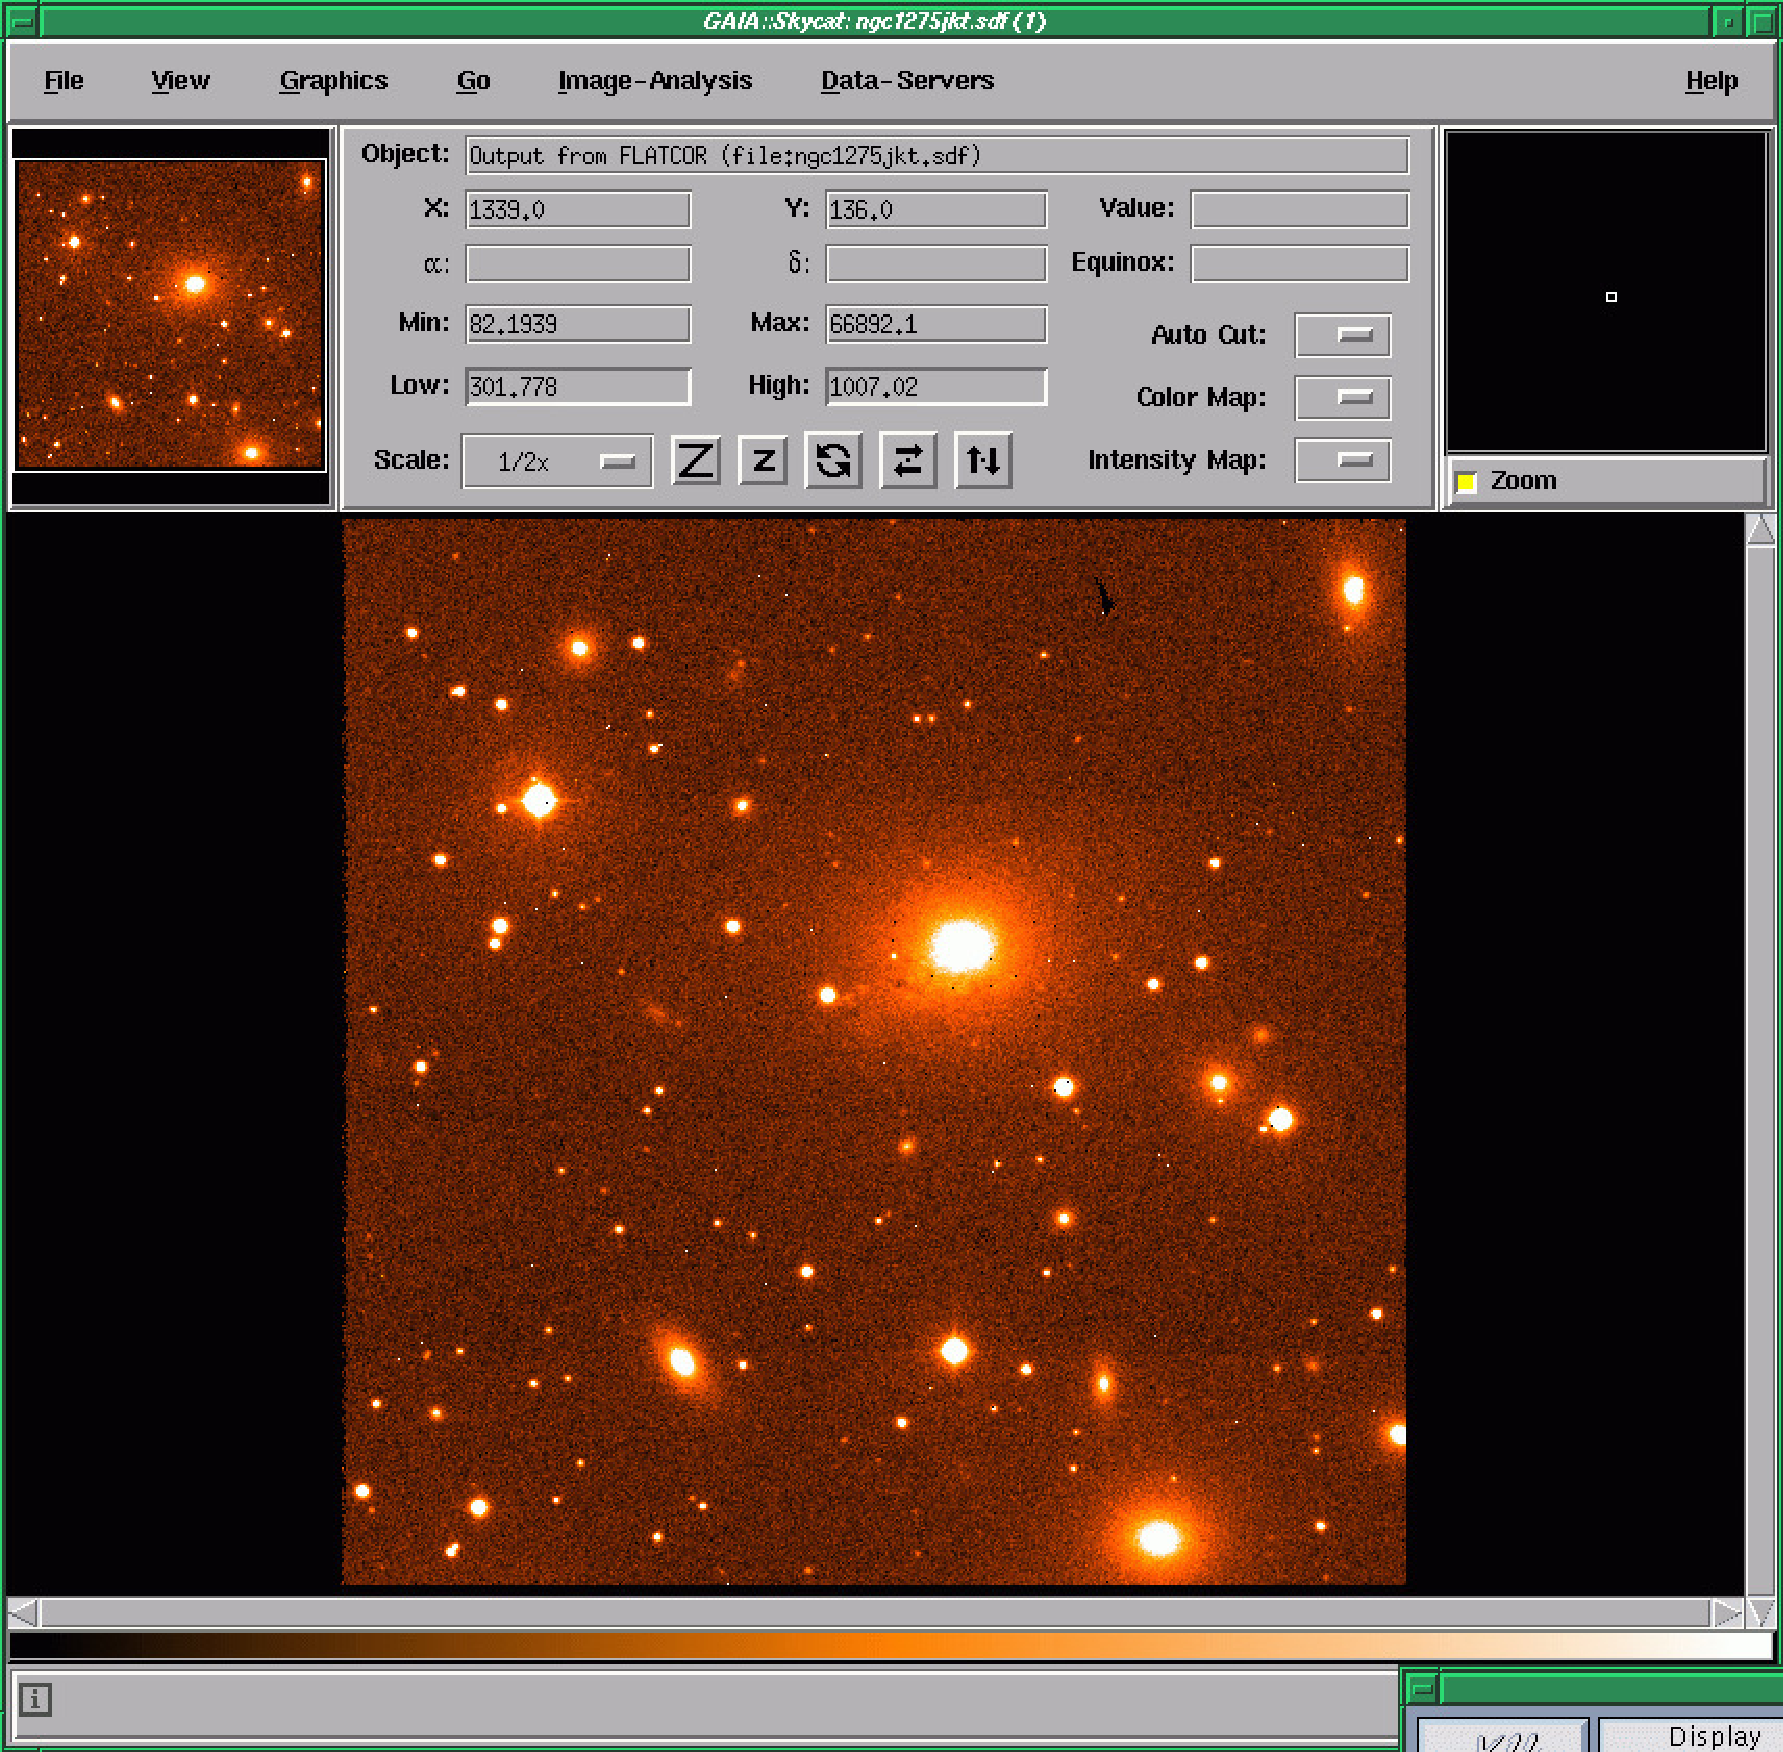
\includegraphics[totalheight=6in]{sc17_disp_r_jkt.ps}
     \begin{quote}
     \caption[A V band CCD image of NGC 1275]
      {A V band CCD image of the galaxy NGC 1275.  The image was obtained
      with the Jacobus Kapteyn Telescope (JKT) on La Palma
     \label{DISP_R_JKT} }
     \end{quote}
  \end{figure}

  \item You can inspect the header information associated with the image
   (see Section~\ref{FORMATS}) by clicking on the {\sf View} menu (second
   on the left on the menu-bar along the top of the main window) and choosing
   the {\sf Fits Header\ldots} option.

   Note that this option will work with images in the NDF format as well
   as those in the FITS format (because the NDF format can contain
   FITS-like header information which GAIA can access).

  \item GAIA has many other functions and options and you may want to spend
   a while exploring some of them.  Similarly, you might also like to
   examine the other images included in the examples.

   On-line help is available from the {\sf Help} menu at the extreme right
   of the menu-bar at the top of the window.  If you click on this menu
   and choose the {\sf Help topics index\ldots} item then the introductory
   page of the GAIA on-line help information will appear (see
   Figure~\ref{DISP_R_HELP}).  From this page you can follow hyper-links
   to further pages giving notes on how to perform numerous common tasks
   with GAIA.  You are likely to find this help information very useful.

  \begin{figure}[htbp]
     \centering
     \includegraphics[totalheight=4in]{sc17_disp_r_help.ps}
     \begin{quote}
     \caption{The introductory GAIA help page
     \label{DISP_R_HELP} }
     \end{quote}
  \end{figure}

  \item When you have finished, close GAIA by clicking on the {\sf File}
   menu and choosing the {\sf Exit} option.

\end{enumerate}


\newpage
\section{\xlabel{RETRIEV_RECIP}\label{RETRIEV_RECIP}Retrieving Remote
Images and Catalogues}

\begin{quote}
{\it When using remote facilities, such as those described in this
recipe, you should ensure that you are both familiar with and comply
with any obligations which they impose on you, such as correct
acknowledgement of the use of data or services \emph{etc}.}
\end{quote}

This recipe demonstrates how to retrieve an image of a specified region
of sky from a remote archive and to overlay it with objects extracted from
a remote catalogue.  In both cases the data are retrieved via the Internet.
As an example a region centered on the galaxy NGC 1275 will be used.
Recall that the J2000 coordinates of this galaxy are:

\begin{center}
% alpha =3:19:48.16,                 delta = +41:30:42.1
$\alpha =$ \hms{3}{19}{48}{16}, ~~ $\delta =$ \dms{+41}{30}{42}{1}
\end{center}

A region will be extracted from the on-line version of the
\htmladdnormallinkfoot{DSS (Digitised Sky Survey)}
{http://stdatu.stsci.edu/dss/}
at ESO.  The DSS is a photographic survey which covers the
entire sky.  It was constructed by the Space Telescope Science Institute
(STScI) by digitising and combining surveys conducted with the Palomar
and UK Schmidt telescopes (a
\htmladdnormallinkfoot{UK mirror}{http://ledas-www.star.le.ac.uk/DSSimage/}
is available as part of the
\htmladdnormallink{LEDAS}{http://ledas-www.star.le.ac.uk/}
data archive service at the
\htmladdnormallink{Department of Physics and Astronomy}
{http://www.star.le.ac.uk/}, University of Leicester).  The DSS image will
then be overlaid with objects extracted from the
\htmladdnormallinkfoot{USNO}{http://www.nofs.navy.mil/} PMM astrometric
catalogue\cite{PMM}.

The \htmladdnormallinkfoot{SuperCOSMOS image surveys}
{http://www-wfau.roe.ac.uk/sss/} also available from GAIA return images
which have catalogues of objects detected in the images already attached
and so combine the two stages into one operation.  However, the SuperCOSMOS
surveys currently only cover the sky south of Declination $+3^{\circ}$.

If the coordinates of your target region or object are not for epoch and
equinox J2000 then you should convert them to this system.  COCO (see
SUN/56\cite{SUN56}) is available for this purpose.  Though the target
coordinates can be converted within GAIA it is probably better to convert
them prior to starting it.

\begin{enumerate}

  \item Start GAIA.  Type:

  \begin{quote}
   {\tt \%  gaia \&}
  \end{quote}

   The ampersand (`{\tt \&}') is simply to run GAIA as a detached process,
   so that you can continue to issue Unix commands from the command line.
   After a few moments the main GAIA window should appear.

  \item The first step is to retrieve a two-dimensional image of the
   region of sky containing your target region or object.  Click on the
   {\sf Data-Servers} menu, located towards the right of the menu-bar at
   the top of the main window.  Choose the {\sf Image Servers} option and
   then {\sf Digitized Sky at ESO} from amongst the list of servers (it
   will probably be the only choice).  If the {\sf Digitized Sky at ESO}
   is not amongst the choices offered then see
   Section~\ref{RESTORE_CONFIG}, below.

  \begin{figure}[htbp]
     \centering
     \includegraphics[totalheight=3in]{sc17_retriev_r_dss.ps}
     \begin{quote}
     \caption[Window to retrieve a remote image]
      {Window to retrieve a remote image of a region or object from the
      DSS
     \label{RETRIEV_R_DSS} }
     \end{quote}
  \end{figure}

   A window similar to Figure~\ref{RETRIEV_R_DSS} and titled {\sf
   Digitized Sky at ESO (1)} should appear; it allows you to specify the
   region of sky to be retrieved.

  \begin{itemize}

    \item You can simply enter the name of your target object in the {\sf
     Object Name:} box, if you know it.  GAIA will attempt to resolve
     the name of the object and look up its coordinates.  Here simply
     enter `{\tt ngc 1275}' (any embedded spaces are ignored).

    \item However, often you will need to enter the coordinates directly.
     The units and formats required are:

    \begin{description}

      \item[$\alpha$] (Right Ascension): sexagesimal hours with a colon
       (`:') as a separator,

      \item[$\delta$] (Declination): sexagesimal degrees with a colon
       (`:') as a separator.

    \end{description}

     In the present example the values required are:

    \begin{description}

      \item[$\alpha${\rm :}] {\tt 3:19:48}

      \item[$\delta${\rm :}] {\tt 41:30:42}

    \end{description}

    \item You also need to specify the height and width of the region to
     be retrieved.  These values are specified in minutes of arc.  In the
     present example values of 7\arcmin should be specified, which is
     slightly larger than the field of view of the V band CCD image of
     NGC 1275 used in the previous recipe (Section~\ref{DISP_RECIP}).

  \end{itemize}

   When the values are set, click on the {\sf Get Image} button.  After
   a few moments the retrieved image should be displayed in the main
   GAIA window.  A small window entitled `{\sf FITS HDUs (1)}' may also
   appear.  Click on {\sf Close} to close this window.  Then click on
   {\sf Close} to close the {\sf Digitized Sky at ESO (1)} window.

  \item You may wish to save the retrieved image as a file for future
   use.  Click on the {\sf File} menu (the leftmost item in the menu-bar
   along the top of the main window) and choose the {\sf Save as\ldots}
   item.  A window allowing you to save the image as a file will appear.
   The file will be written in FITS format.  It is usual to end the
   file-name with a file-type of `{\tt .fits}' or `{\tt .fit}'.

  \item You may wish to adjust the appearance of the displayed image.
   The most likely items to change are {\sf Colors\ldots} and {\sf
   Magnification} in the {\sf View} menu (second from the left in the
   menu-bar along the top of the window).

   For example, click on the {\sf View} menu and select the {\sf
   Colors\ldots} option.  A panel will appear.  Set:

  \begin{itemize}

    \item the colour scale algorithm to {\sf Linear},

    \item the colormap to {\sf ramp},

    \item the intensity to {\sf neg}.

  \end{itemize}

   Then click on the {\sf Close} button.
   Set the magnification by clicking on the {\sf Scale:} button (in the
   bottom left of the control panel in the centre top of the window) and
   setting it to {\sf 2x}.

   The display should now look something like Figure~\ref{RETRIEV_R_MAIN},
   which is a a reasonable approximation to the appearance of the
   original photographic plate.

  \begin{figure}[htbp]
     \centering
     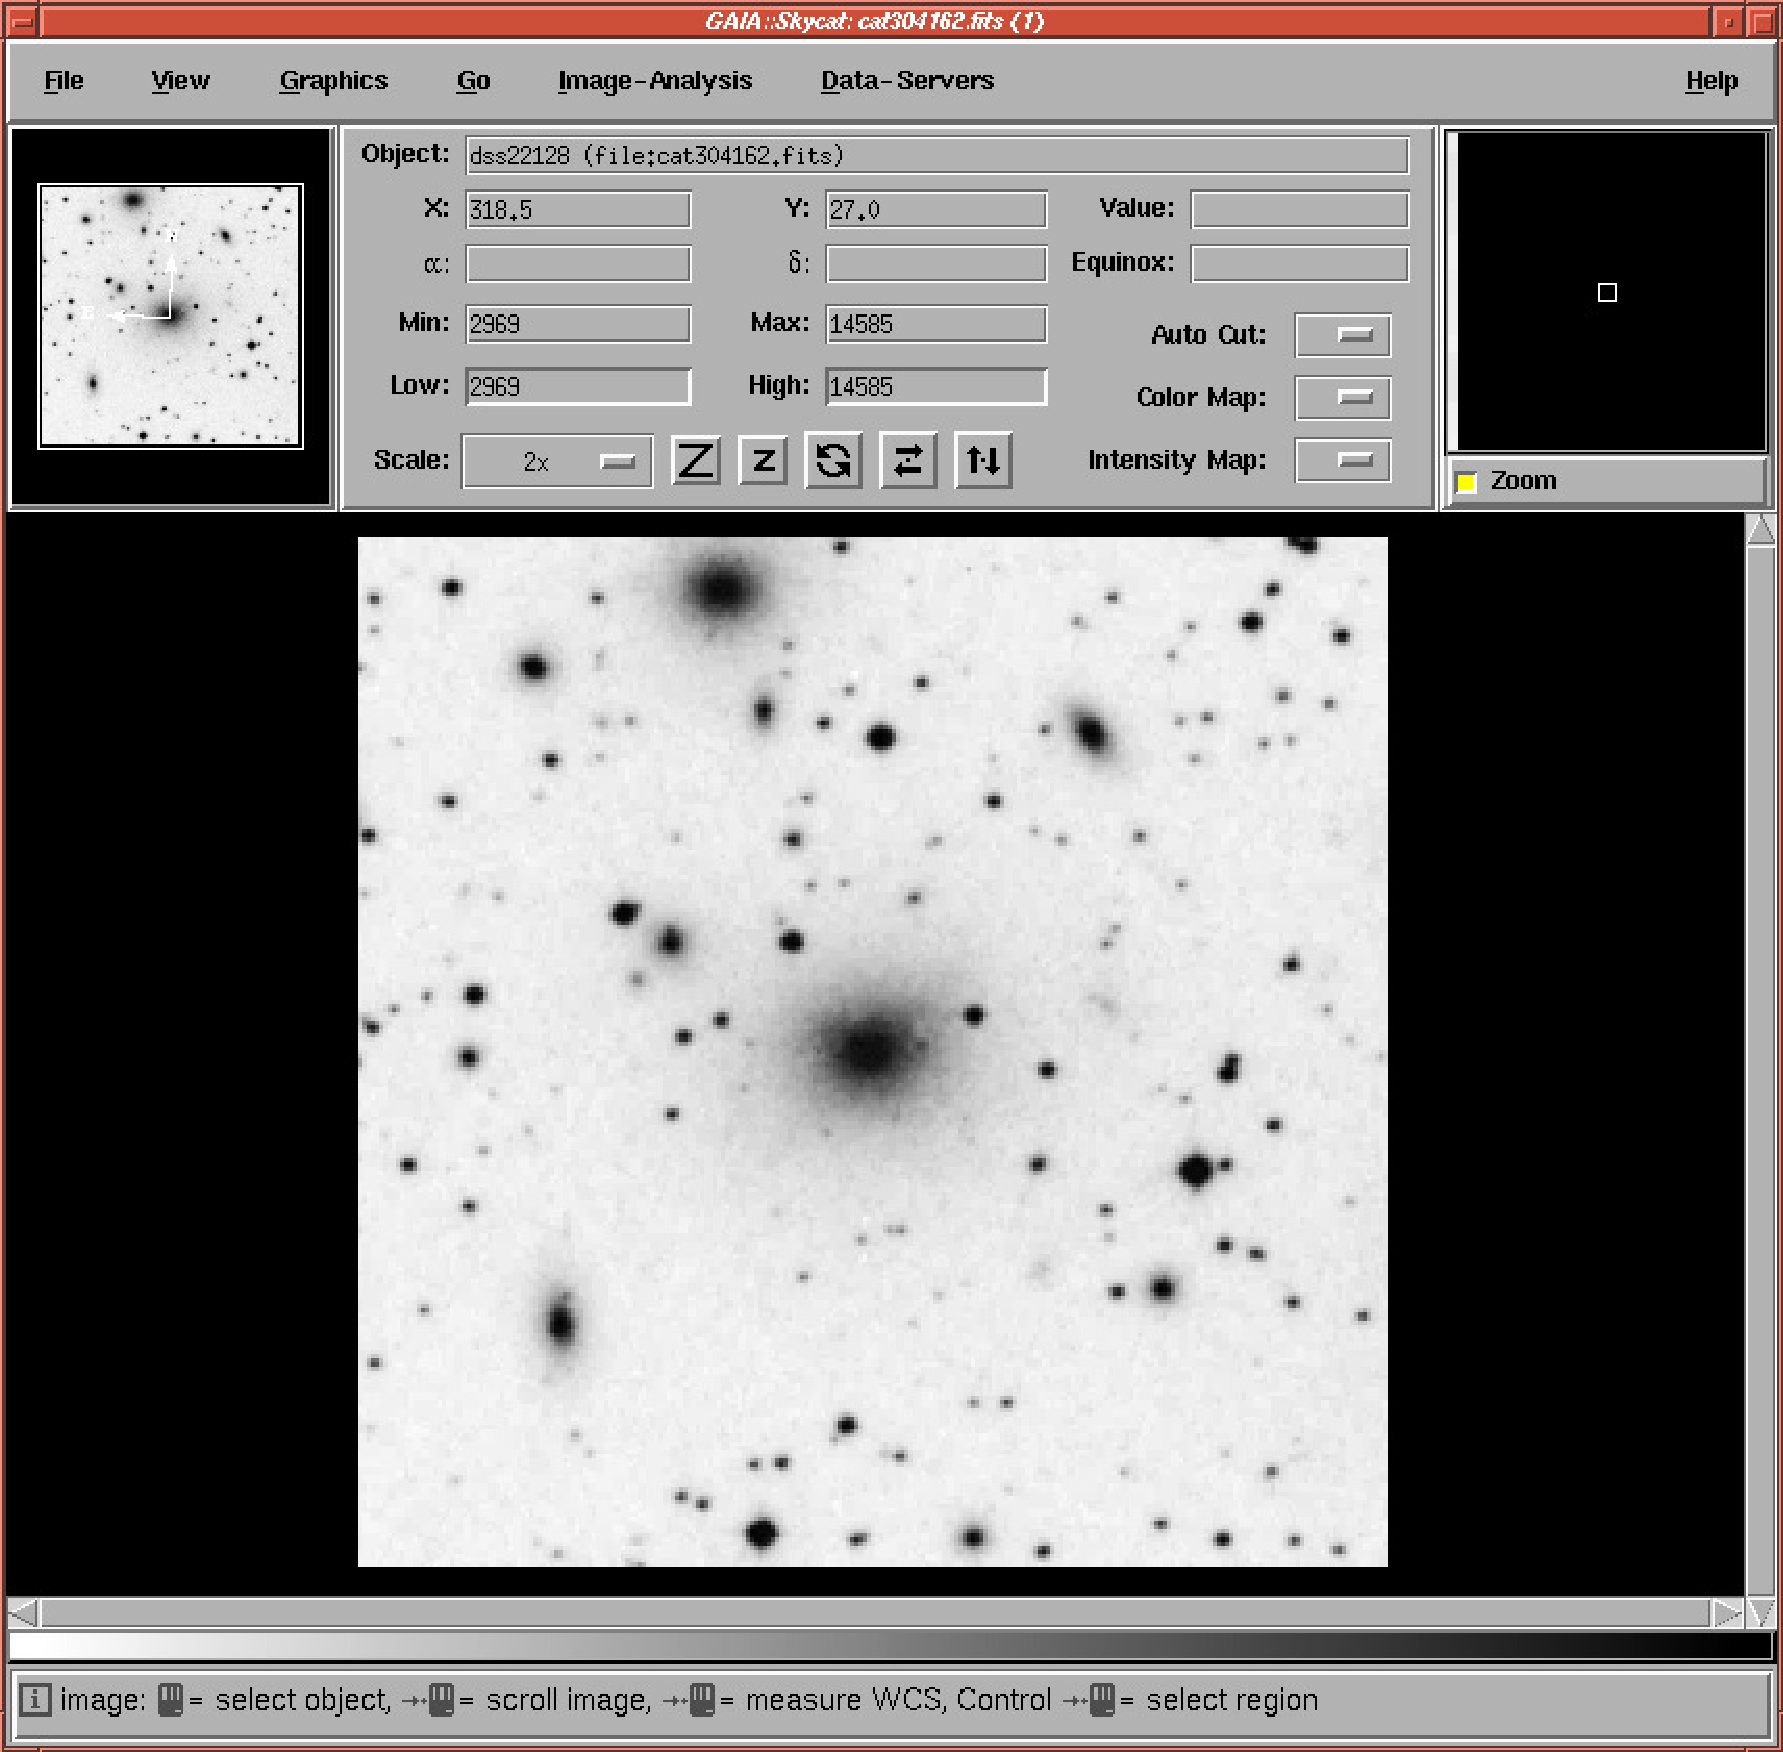
\includegraphics[totalheight=5in]{sc17_retriev_r_main.ps}
     \begin{quote}
     \caption[Retrieved DSS image centred on NGC 1275]
     {Retrieved Digitised Sky Survey (DSS) image centred on NGC 1275
     \label{RETRIEV_R_MAIN} }
     \end{quote}
  \end{figure}

  \item Various remote catalogues are accessible from GAIA.  The present
   recipe extracts objects from the
   \htmladdnormallinkfoot{USNO}{http://www.nofs.navy.mil/} PMM astrometric
   catalogue\cite{PMM} and overlays them on the image.

   First click on the {\sf Data-Servers} menu, towards the right of the
   menu-bar at the top of the main window.  Choose the {\sf Catalogs}
   option and then {\sf USNO at ESO} from amongst the list of catalogues
   (it will probably be towards the bottom of the list).  If {\sf USNO at
   ESO} is not amongst the choices offered then see
   Section~\ref{RESTORE_CONFIG}, below.

   A window similar to Figure~\ref{RETRIEV_R_PMM} and titled {\sf USNO at
   ESO (1)} should appear; it allows you to retrieve objects from the
   catalogue.  The central position and minimum and maximum radius should
   be already filled in (the values have been obtained from the
   two-dimensional image).  The `{\sf Brightest (min):}' and `{\sf Faintest
   (max):}' boxes allow these quantities to be set, if desired.  However,
   in the present example they can be left blank, and all the objects in
   the PMM which overlay the image will be selected.

  \begin{figure}[htbp]
     \centering
     \includegraphics[totalheight=4in]{sc17_retriev_r_pmm.ps}
     \begin{quote}
     \caption[Window to retrieve a remote catalogue]
      {Window to retrieve objects from a remote version of the USNO
      PMM catalogue
     \label{RETRIEV_R_PMM} }
     \end{quote}
  \end{figure}

   Simply click on the {\sf Search} button (in the bottom left of the
   window).  After a couple of moments the selected objects are listed
   in the {\sf Search Results} box and overlaid on the image in
   the main window.

   A useful feature for identifying objects in the list with the
   corresponding plotted symbol is that if you position the cursor over
   either a plot symbol or a row in the table and click with the left
   mouse button the corresponding row and plot symbol are highlighted.

   To save the selected objects as a text file click on the {\sf File}
   menu in the {\sf USNO at ESO (1)} window (the leftmost item in its
   menu-bar) and choose either {\sf Save as\ldots} or {\sf Print\ldots}.
   In both cases a window will appear which allows you to save the list.
   Note that though both options produce text files they are in different
   formats.

   If you choose the {\sf Save as\ldots} option the catalogue of objects
   will be saved as a file.  The format in which this catalogue is saved
   depends on the    file-type specified at the end of the file-name (see
   Section~\ref{CATS}).  Catalogues saved in the FITS tables, TST or STL
   formats can subsequently be imported into CURSA (see
   \xref{SUN/190}{sun190}{}\cite{SUN190}) which provides additional
   catalogue manipulation facilities.

   When you have finished click the {\sf Close} button to close the {\sf
   USNO at ESO (1)} window.

  \item To close GAIA click on the {\sf File} menu (the leftmost item in
   the menu-bar along the top of the main window) and choose the {\sf
   Exit} option.

\end{enumerate}

\subsection{\label{RESTORE_CONFIG}Restoring catalogue access}

It is possible to configure the set of catalogues and sky surveys which
GAIA can access, though the details are not germane here.  However, if
the {\sf Digitized Sky at ESO} survey or {\sf USNO at ESO} catalogue do
not appear in the lists of {\sf Image Servers} and {\sf Catalogs}
respectively then the most likely reason is that the default list of
catalogues and surveys has been substituted with one which does not
include them.  The simplest way to restore access is to revert to using
the default list.  GAIA configuration files are kept in subdirectory {\tt
.skycat} of your top level directory.  To restore the default catalogues
and surveys you should delete (or rename) file:

\begin{center}
\verb+~/.skycat/skycat.cfg+
\end{center}

and then restart GAIA.

\subsection{Using a proxy server}

Access to the World Wide Web at your site may be restricted (by a firewall
or maybe just by policy), so that it is only available through a `web cache'
or proxy server.  If you are in this situation you will need to configure
GAIA so that its remote catalogue access will work.  Proceed as follows.

\begin{enumerate}

  \item Start GAIA, select the {\sf Data-Servers} menu (in the menu-bar
   along the top of the main window) and choose any remote catalogue.

  \item The catalogue window will appear (similar to
   Figure~\ref{RETRIEV_R_PMM}).  Click on the {\sf Options} menu in its
   menu-bar and choose the {\sf Proxies\ldots} item.

  \item a {\sf Proxies} window will appear.  You should fill in the various
   fields (consult your system manager if you are unsure what to enter).
   Then click on {\sf OK}.

\end{enumerate}


\newpage
\section{\xlabel{WCS_RECIP}\label{WCS_RECIP}Using World Coordinates}

This recipe demonstrates the simple use of World Coordinates in GAIA.
Recall that a World Coordinate System (WCS; see Section~\ref{WCS})
relates the positions of pixels in an image to celestial coordinate
systems on the sky.  In practice it allows you to display and annotate
images in terms of celestial coordinates.

Some images include a WCS as part of the auxiliary information that they
contain; others do not.  For example, {\tt ngc1275jkt.sdf}, the JKT image
used in the recipe in Section~\ref{DISP_RECIP} does not possess a WCS,
but images retrieved from the DSS (as in the recipe in
Section~\ref{RETRIEV_RECIP}) do.  It is possible to use GAIA to add a WCS
to an image, and the recipe in Section~\ref{ASTROM_RECIP} is an example
doing so.  The present recipe merely gives some examples of using a WCS.

The recipe uses file {\tt ngc1275dss.sdf} which is an image centred on
the galaxy NGC 1275 extracted from the DSS.  It will be very similar to
the image that you created in the recipe in Section~\ref{RETRIEV_RECIP},
and you could substitute your own image if you prefer.

Load file {\tt ngc1275dss.sdf} into GAIA and adjust the colour table
so that you can see the stars and galaxies.  The display should look
something like Figure~\ref{RETRIEV_R_MAIN}.

\subsection{Reading off the Right Ascension and Declination}

It is straightforward to read off the approximate Right Ascension and
Declination of any object in the image.

\begin{enumerate}

  \item The $x,y$\/ pixel positions and the Right Ascension and Declination
   of the current cursor position are shown in the boxes labelled: {\sf
   X:}, {\sf Y:}, {\sf $\alpha$:} and {\sf $\delta$:} in the control panel
   in the middle of the upper portion of the main window.  To find the
   approximate coordinates of a star simply position the cursor over it and
   read them off.

  \item In a DSS image J2000 equatorial coordinates are shown by default.
   It is possible to configure GAIA to display other celestial coordinates.
   Click on the {\sf Image-Analysis} button in the menu-bar along the top
   of the main window and choose {\sf Change coordinates} and then
   {\sf Celestial coordinates\ldots}.

   A window appears which allows you to specify the coordinate system.
   Choose the one required (perhaps {\sf ecliptic} coordinates) and then
   click the {\sf Accept} button.

   Henceforth coordinates are displayed in the chosen system (but note
   that the coordinate boxes are still labelled `{\sf $\alpha$:}' and
   `{\sf $\delta$:}', even if ecliptic or Galactic coordinates have been
   selected).

   Also, the coordinates are only updated when the cursor moves.  Thus,
   if it is already positioned over the star that you are interested in,
   then you need to nudge it off the object and return it to the required
   position.

  \item Depressing the {\tt Caps Lock} key will prevent the $x,y$\/ and
   $\alpha$,$\delta$\/ values being updated as the cursor moves.  This
   facility is useful, for example, if you wish to preserve the coordinates
   whilst moving the cursor to another window.

  \item A list of positions in an image can be selected and saved as a text
   file by selecting the {\sf Positions\ldots} item from the {\sf
   Image-Analysis} menu (in the menu-bar along the top of the main window).

\end{enumerate}

\subsection{Showing celestial coordinate grids}

GAIA can superimpose a celestial coordinate grid over the image.

\begin{enumerate}

  \item Click on the {\sf Image-Analysis} button in the menu-bar along
   the top    of the main window and choose {\sf Overlay axes grid\ldots}.
   A window will appear with numerous options.  You can change some of
   these if you wish, but there is no need to do so.  Simply click on the
   {\sf Draw} button and an axis grid is drawn in the current celestial
   coordinate system.

   The grid is removed when you click {\sf Close} to close the window.

  \item To show a grid in a different celestial coordinate system click
   on the {\sf Image-Analysis} button in the menu-bar along the top
   of the main window and choose {\sf Change coordinates} and then
   {\sf Celestial coordinates\ldots}.  A window appears which allows you
   to specify the coordinate system.  Choose the one required and then
   click the {\sf Accept} button.

   Then repeat step 1, above, and a grid will be drawn in the new system.

\end{enumerate}

\subsection{Measuring angular separation}

To measure the approximate angular separation between two objects simply
position the cursor over the first of them, and then click and hold down
mouse button three.  Continuing to hold down this mouse button, move the
cursor until it is positioned over the second object.

A `rubber band' cursor is drawn as the mouse moves.  It shows the vector
between the original and current positions and also the offsets in two
orthogonal coordinates.  The separation and offsets are all labelled with
their size in minutes of arc, with a sexagesimal subdivision into seconds.

The cursor disappears when the mouse button is released.


\newpage
\section{\xlabel{SUPER_RECIP}\label{SUPER_RECIP}Superimposing and
Contouring Images}

This recipe is an example of superimposing two images in order to compare
them.  GAIA has two mechanisms for superimposing images: displaying two
or more images and rapidly blinking between them (in a manner analogous to
the `blink comparator' used to compare photographic plates), and displaying
one image as a set of contours superimposed on a display of the other.
This recipe demonstrates the latter technique.

GAIA aligns images by using their World Coordinate Systems (WCS; see
Section~\ref{WCS}).  Images that do not have a WCS are aligned by assuming
that their pixel coordinates are coincident, which can be useful in some
circumstances.  Images extracted from the Digitised Sky Survey (DSS) have
a WCS, and this recipe will use the DSS image of NGC 1275 retrieved in
Section~\ref{RETRIEV_RECIP}.  Contours constructed from an X-ray image of
the same region of sky will be drawn on top of it.  The X-ray image is
contained in file {\tt ngc1275hri.fits}.  It was obtained with the HRI (High
Resolution Imager) on-board the ROSAT X-ray astronomy satellite ({\it
R\"{o}ntgensatellit}\/).  The copy used here was retrieved from the
\htmladdnormallinkfoot{LEDAS}{http://ledas-www.star.le.ac.uk/}
data archive service at the
\htmladdnormallink{Department of Physics and Astronomy}
{http://www.star.le.ac.uk/}, University of Leicester.  The image is in
FITS format (see Section~\ref{FORMATS} for details of the data formats
available to GAIA) and it too contains a WCS.

Proceed as follows.

\begin{enumerate}

  \item It is useful to examine the X-ray image of the NGC 1275 region
   before trying to contour it.  (You could skip these steps if you
   were already familiar with the properties of the image to be contoured).
   Start GAIA and load file {\tt ngc1275hri.fits}.

  \item Adjust the colour so that the very nucleus of the X-ray emission
   is clearly visible.  For example, set the {\sf Auto Cut:} to 100\%.
   Then click on the {\sf View} menu and select the {\sf
   Colors\ldots} option.  A panel will appear.  Set the colour scale
   algorithm to {\sf Logarithmic}, the colormap to {\sf heat} and the
   intensity to {\sf ramp}.  The display should now appear similar to
   Figure~\ref{SUPER_R_HRI}.

   It is immediately obvious that the sky appears very different at X-ray
   and optical wavelengths.  Also, by moving the cursor from one edge of
   the image to the other and noting the change in Right Ascension or
   Declination it is apparent that the image is rather larger than the
   7\arcmin field extracted from the DSS.

  \begin{figure}[htbp]
     \centering
     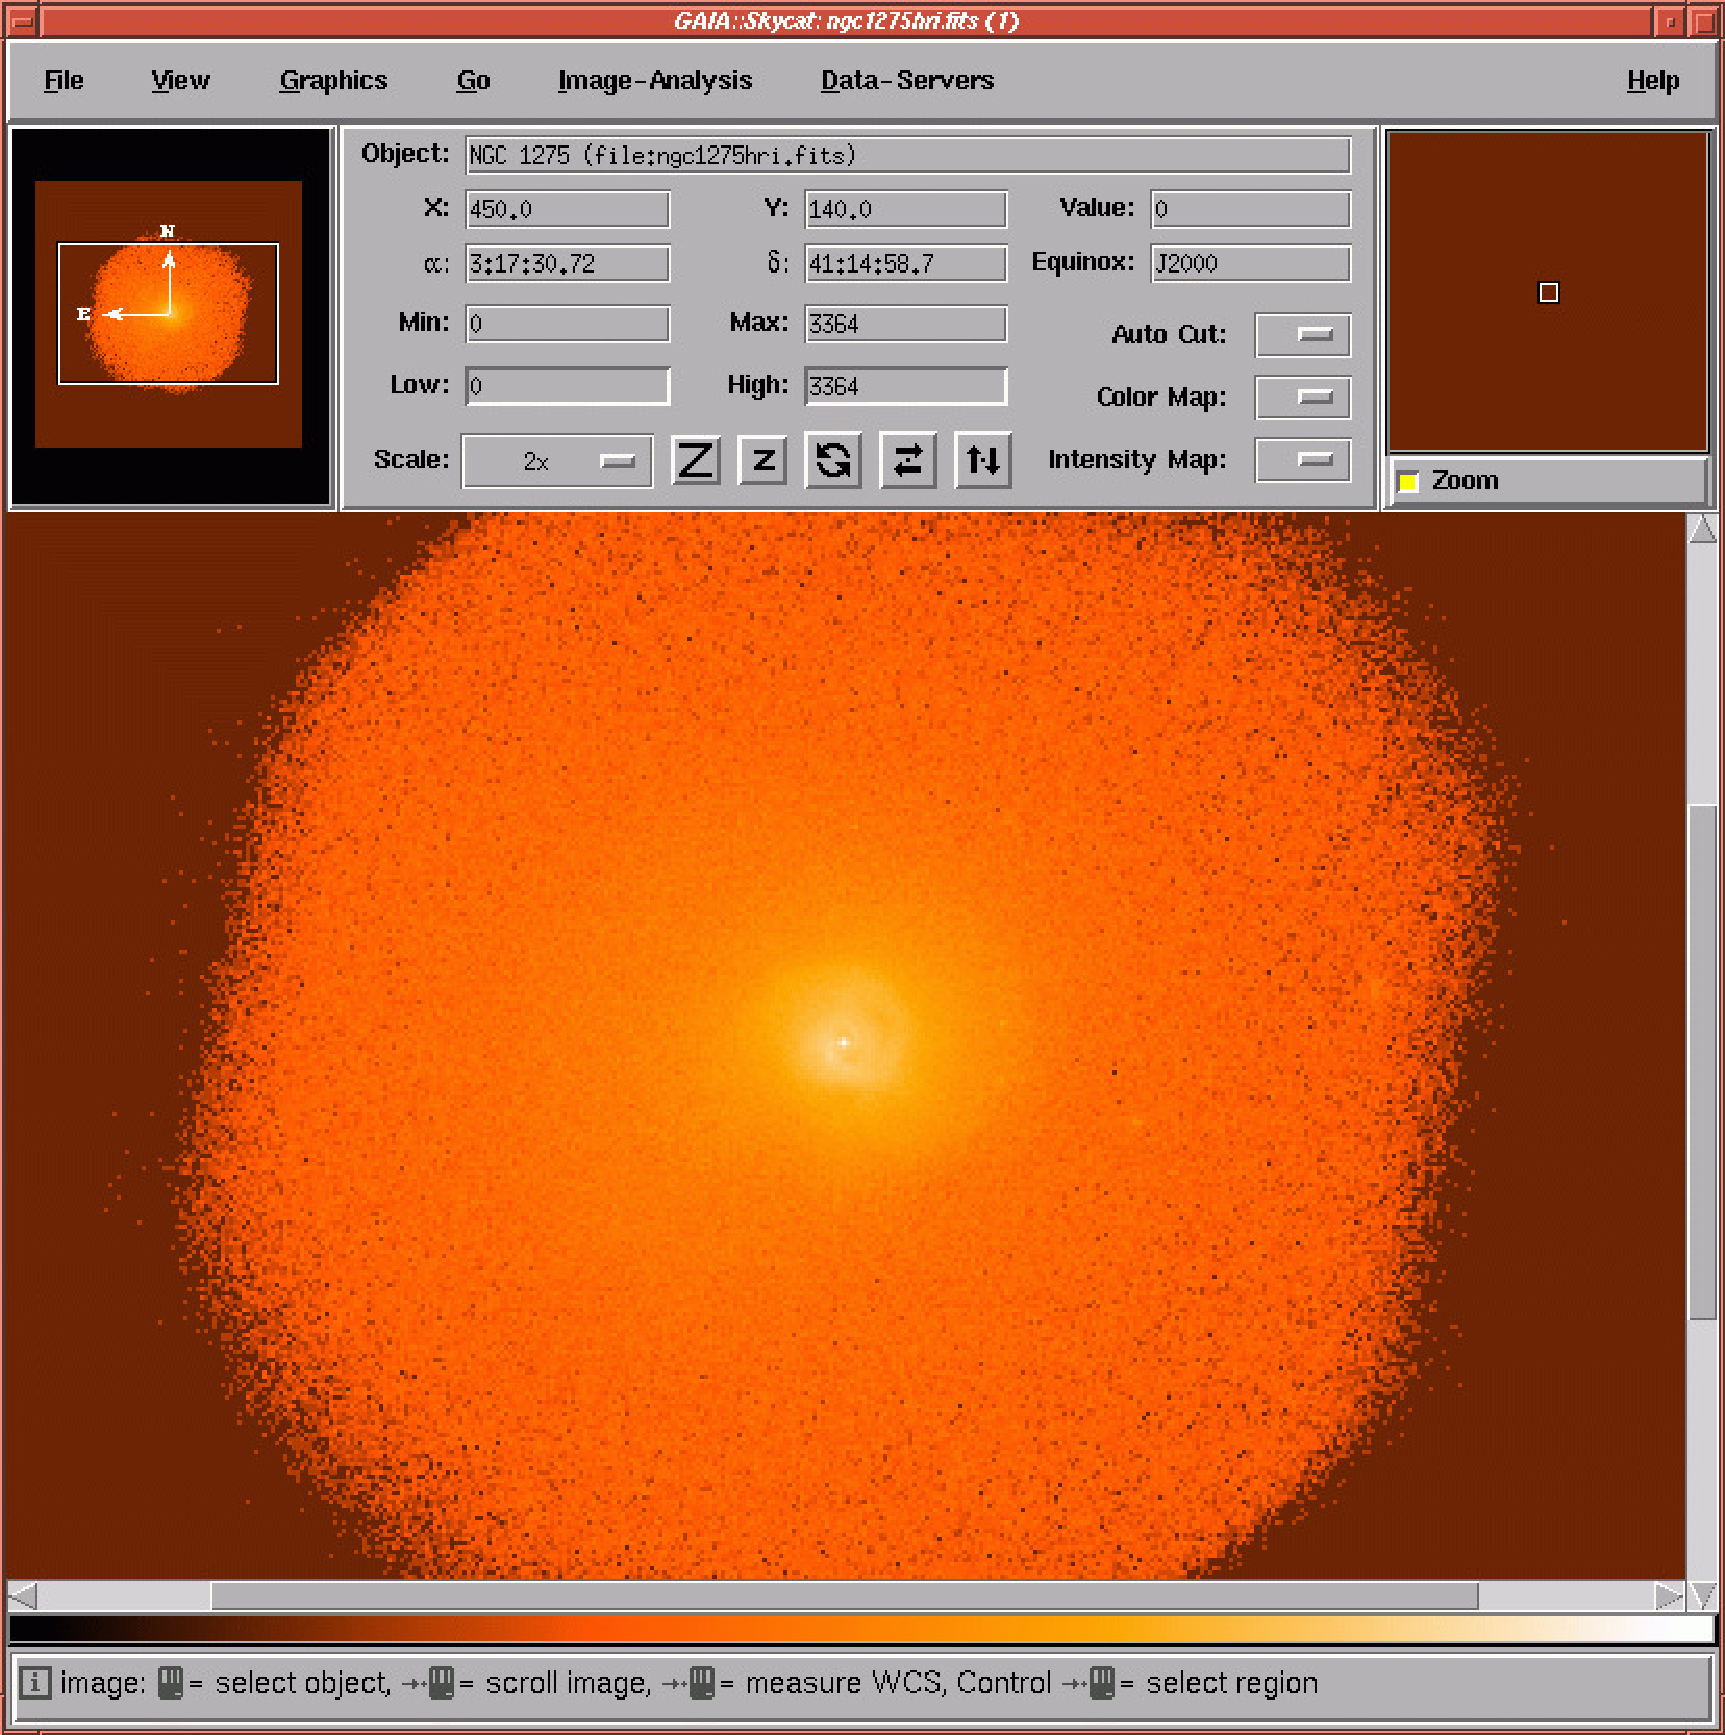
\includegraphics[totalheight=6in]{sc17_super_r_hri.ps}
     \begin{quote}
     \caption[An X-ray image of NGC 1275]
      {An X-ray image centred on the galaxy NGC 1275.  The image was
      obtained with the HRI instrument on the ROSAT satellite
     \label{SUPER_R_HRI} }
     \end{quote}
  \end{figure}

  \item {\bf Aside:} you might be interested to check that the X-ray
   image really is centred on NGC 1275.

  \begin{enumerate}

    \item Click on the {\sf Data-Servers} menu, towards the right of the
     menu-bar at the top of the main window and choose the {\sf Catalogs}
     option.  Select the {\sf RC3 at CADC} catalogue, which is a version
     of the {\it Third Reference Catalogue of Bright Galaxies}\/\cite{RC3}
     provided by the
     \htmladdnormallinkfoot{CADC (Canadian Astronomy Data Center)}
     {http://cadcwww.dao.nrc.ca/}.

     A window similar to Figure~\ref{RETRIEV_R_PMM} should appear.  Click
     on the {\sf Search} button (in the bottom left of the window) and
     after a couple of moments the galaxies in the RC3 which overlay the
     X-ray image will be listed in the {\sf Search Results} box and plotted
     in the main window.

    \item One of the plotted objects is almost exactly coincident with the
     centre of the X-ray emission.  If you click on this symbol the line
     for NGC 1275 is highlighted in the {\sf Search Results} box.

    \item If you double-click on the line for NGC 1275 in the {\sf Search
     Results} box the corresponding symbol in the image is labelled as
     NGC 1275.

  \end{enumerate}

  \item Before contouring an image it is useful to have some idea of the
   range of numbers that it contains.  One possibility is to draw a slice
   through the image.  Click on the {\sf View} button on the menu-bar
   along the top of the main window and choose the {\sf Slice\ldots} item.
   You can interactively define a slice through the image which is then
   plotted as a graph (see Figure~\ref{PHOTOM_R_SLICE} in
   Section~\ref{PHOTOM_RECIP}, below, for an example).

   Alternatively, click on the {\sf View} button on the menu-bar
   along the top of the main window and choose the {\sf Pixel Table\ldots}
   item.  A table showing the values of a small grid of pixels centred on
   the current  cursor position is displayed.  You can move the cursor over
   the image examining the values.  For the present purposes the largest
   grid permitted, {\sf 9x9}, is the most appropriate.

   You will probably want to experiment with these options for a while.

  \item You are now ready to proceed with contouring the X-ray image on top
   of the DSS one.  Load the DSS image {\tt ngc1275dss.sdf} into GAIA.  If
   you prefer you can substitute the DSS image that you retrieved whilst
   working through the recipe in Section~\ref{RETRIEV_RECIP}; they should
   be very similar.

  \item Set the colour table and magnification as in
   Section~\ref{RETRIEV_RECIP}: click on the {\sf View} menu and select
   the {\sf Colors\ldots} option.  Set the colour scale algorithm to {\sf
   Linear}, the colormap to {\sf ramp} and the intensity to {\sf neg}.
   Then click on the {\sf Close} button.

   Set the magnification by clicking on the {\sf Scale:} button (in the
   bottom left of the control panel in the centre top of the window) and
   setting it to {\sf 2x}.

   The appearance of the display should now be similar to
   Figure~\ref{RETRIEV_R_MAIN}.

  \item Click on the {\sf Image-Analysis} button on the menu-bar along the
   top of the main window and choose the {\sf Contouring\ldots} item.
   A window similar to Figure~\ref{SUPER_R_CONT} should appear.

  \begin{figure}[htbp]
     \centering
     \includegraphics[totalheight=3.5in]{sc17_super_r_cont.ps}
     \begin{quote}
     \caption{Window for defining contour details
     \label{SUPER_R_CONT} }
     \end{quote}
  \end{figure}

  \item Click on the {\sf Choose file\ldots} button and load file {\tt
   ngc1275hri.fits}.

  \item Click on the {\sf Generate} button (on the left hand side of the
   window, immediately below {\sf Levels}).  A window similar to
   Figure~\ref{SUPER_R_LEVELS} should appear.  Set the following values:

  \begin{center}
  \begin{tabular}{rl}
   {\sf Number:}    & {\tt 5} \\
   {\sf Algorithm:} & {\tt linear} \\
   {\sf Start:}     & {\tt 100} \\
   {\sf Increment:} & {\tt 75} \\
  \end{tabular}
  \end{center}

   The window should now appear exactly like Figure~\ref{SUPER_R_LEVELS}.
   (In this recipe the required contour levels are already prescribed,
   however, the first time you contour an image you will probably need
   to experiment to find suitable levels.  One way to do so is to set the
   {\sf Algorithm:} to {\sf automatic} and allow GAIA to generate the
   levels itself.  If these levels are not satisfactory you can adjust
   them manually.)

  \begin{figure}[htbp]
     \centering
     \includegraphics[totalheight=3.5in]{sc17_super_r_levels.ps}
     \begin{quote}
     \caption{Window for defining contour levels
     \label{SUPER_R_LEVELS} }
     \end{quote}
  \end{figure}

   Click on the {\sf Generate} button and the appearance of the window
   should revert to that in Figure~\ref{SUPER_R_CONT}.

  \item For all five of the specified contours click on the colour boxes
   and set them to red (which makes the contours easier to see if you are
   using the colour table set up above).

  \item Click on the {\sf Draw Contours} button.  Contours of the X-ray
   image will now be drawn superimposed on the X-ray image.  The
   appearance of the plot should be similar to Figure~\ref{SUPER_R_SUPER}.

  \begin{figure}[htbp]
     \centering
     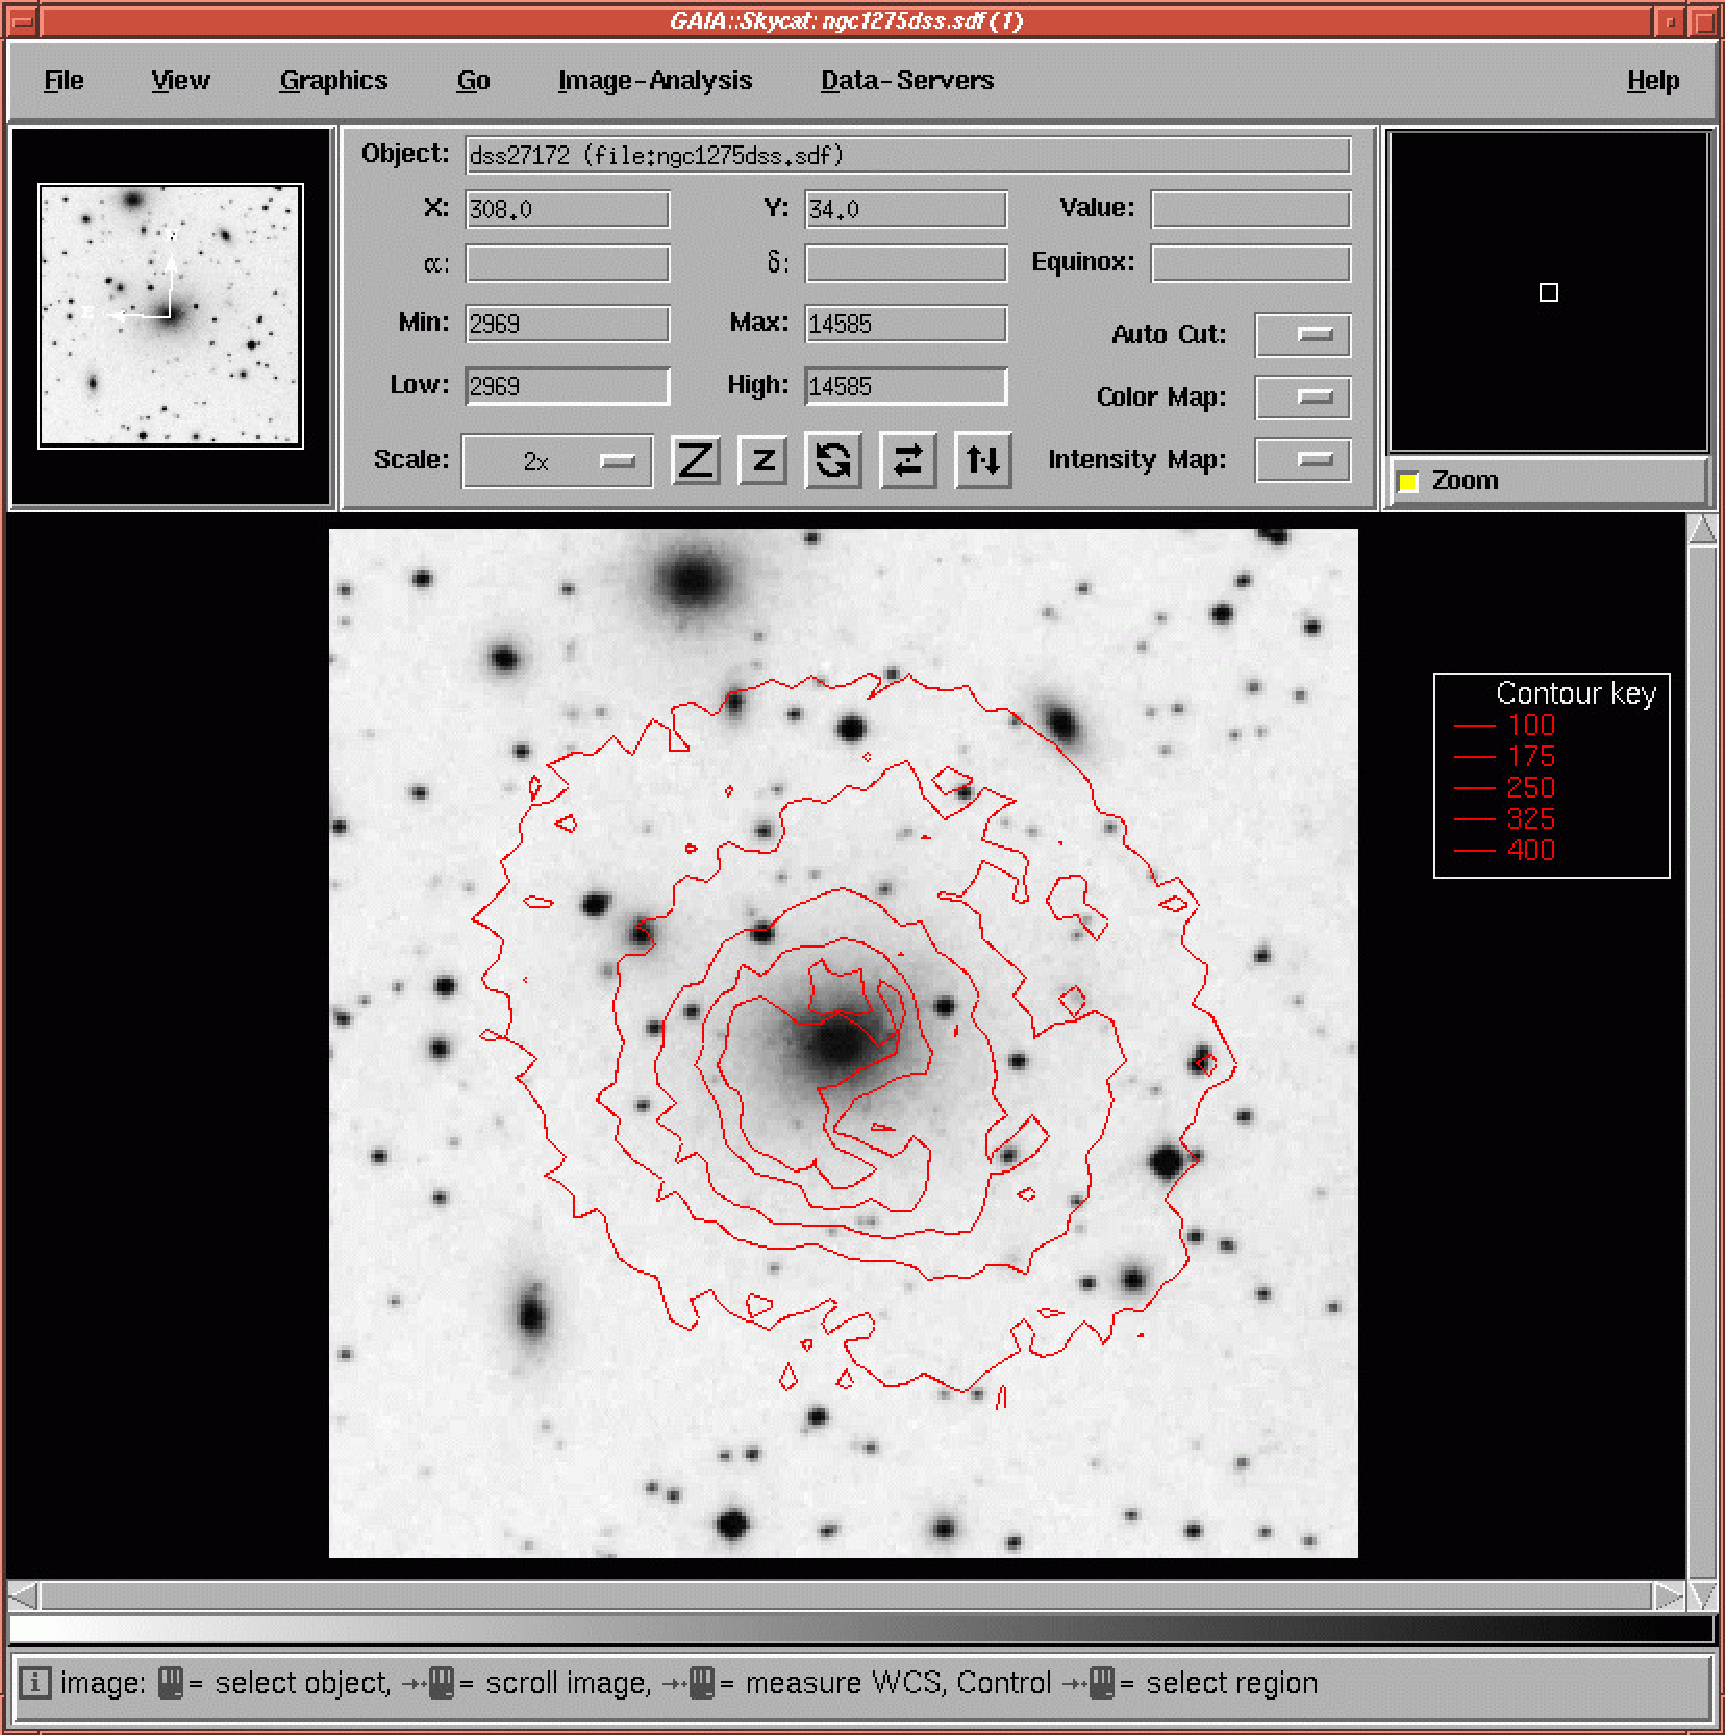
\includegraphics[totalheight=6in]{sc17_super_r_super.ps}
     \begin{quote}
     \caption[X-ray contours superimposed a DSS image of NGC 1275]
      {Contours derived from the ROSAT HRI X-ray image of NGC 1275
      superimposed on a DSS image of the same region
     \label{SUPER_R_SUPER} }
     \end{quote}
  \end{figure}

   It is immediately obvious that the X-ray emission is centred on NGC
   1275 and also that it extends beyond the optical limits of the
   galaxy (recall that the faintest contour drawn corresponds to quite
   a bright level in the X-ray image).

  \item When you have finished inspecting the image click on the {\sf
   Close} button and the contours will disappear.

\end{enumerate}

\subsection{Contouring the displayed image}

Sometimes you might wish to plot contours generated from the displayed
image, rather than superimposing those from another image.  The procedure
is very similar.

\begin{enumerate}

  \item Display the required image.

  \item Click on the {\sf Image-Analysis} button on the menu-bar along the
   top of the main window and choose the {\sf Contouring\ldots} item, as
   before.  A window similar to Figure~\ref{SUPER_R_CONT} should appear.

  \item Do not click on the {\sf Choose file\ldots} button to specify
   the image to be contoured.  Rather, proceed immediately to specifying
   and generating the contour levels by clicking on the {\sf Generate}
   button and then proceed as before.

\end{enumerate}


\newpage
\section{\xlabel{ASTROM_RECIP}\label{ASTROM_RECIP}Astrometric Calibration}

This recipe describes how to apply an astrometric calibration to an
image.  In this context an `astrometric calibration' is a mathematical
transformation relating the $x,y$\/ positions of pixels in the image
array to celestial coordinates on the sky.  Applying an astrometric
calibration is just another term for creating a World Coordinate System
(WCS; see Section~\ref{WCS}) for the image, with the World Coordinates
being celestial coordinates.

GAIA provides numerous options for astrometric calibration, only one of
which will be used here (though Section~\ref{VARIAT}, below, gives a few
hints about what else is available).  In most of the techniques stars
occurring in the image are used as fiducial marks and a transformation is
defined between their $x,y$\/ pixel positions measured in the image and
their celestial coordinates obtained from an astrometric reference
catalogue.  The most interactive (and problematic) part of the procedure
is identifying a given object in the image with the corresponding entry in
an astrometric reference catalogue.

The principal information which you need to know about an image before
attempting astrometric calibration is the approximate position on the sky
corresponding to the centre of the image and the size of the field of view.
The former can usually be obtained from examining the auxiliary information
included with the image (see Section~\ref{FORMATS}).  The latter may also
be found in the auxiliary information or from the documentation for the
instrument or telescope.  If you have no prior information whatsoever
about the region of sky observed then astrometric calibration will usually
be impossible.

In this recipe an astrometric calibration will be created for the V band
CCD image of NGC 1275 obtained with the JKT which was used in the recipe
in Section~\ref{DISP_RECIP}.  The field of view of this image is about
six minutes of arc in each axis.

The process of creating the astrometric calibration divides naturally
into three stages:

\begin{enumerate}

  \item finding suitable astrometric reference stars,

  \item creating a preliminary astrometric calibration,

  \item creating a final accurate astrometric calibration.

\end{enumerate}

Each stage is described separately in individual sub-recipes below.

\subsection{Finding astrometric reference stars}

The purpose of this stage is to find a small number of astrometric
reference stars, imaged on the CCD frame, which can be used to define the
preliminary astrometric calibration.  Traditionally finding reference
stars is a long-winded task involving consulting printed atlases and
catalogues.  However, the on-line resources available to GAIA allow the
process to be automated and simplified.  Proceed as follows.

\begin{enumerate}

  \item You need to extract a region of the Digitised Sky Survey (DSS)
   roughly corresponding to the region imaged in the CCD frame.  The
   first part of the recipe in Section~\ref{RETRIEV_RECIP} gives exactly
   the procedure required.  Either: repeat this procedure, load the image
   that you created when previously working through
   Section~\ref{RETRIEV_RECIP} into GAIA, or load file {\tt ngc1275dss.sdf}
   into GAIA (the last is the required region, already extracted from
   the DSS).

  \item Adjust the colour table until the image appears as in
   Figure~\ref{RETRIEV_R_MAIN}.  Click on the {\sf View} menu and select
   the {\sf Colors\ldots} option.  A panel will appear.  Set the colour
   scale algorithm to {\sf Linear}, the colormap to {\sf ramp} and the
   intensity to {\sf neg}.  Then click on the {\sf Close} button.

   Set the magnification by clicking on the {\sf Scale:} button (in the
   bottom left of the control panel in the centre top of the window) and
   setting it to {\sf 2x}.

  \item Overlay the DSS image with objects selected from the {\sf USNO at
   ESO} catalogue, following the second part of the recipe in
   Section~\ref{RETRIEV_RECIP}.

  \item The next step is to choose five stars in the image to act as
   reference stars.  These stars should be:

  \begin{itemize}

    \item easily identified,

    \item reasonably bright,

    \item stars rather than galaxies (because star images have more
     precisely defined centres),

    \item isolated from other stars and galaxies (to avoid images which
     blend together),

    \item spread reasonably uniformly over the image,

    \item not very close to the edge of the image (later you will need to
     to identify the corresponding stars in the JKT image, and the two
     areas of sky are not exactly the same).

  \end{itemize}

   Figure~\ref{ASTROM_R_PAPER} shows five suitable stars in the DSS
   example image.  To select the stars: hold down the {\tt shift} key and
   click on each star in turn (without releasing the {\tt shift} key).  As
   you do so the selected star is highlighted in both the image and the
   catalogue windows.  You can add as many stars as you like, but five is
   adequate.

  \begin{figure}[htbp]
     \centering
     \includegraphics[totalheight=6in]{sc17_astrom_r_paper.ps}
     \begin{quote}
     \caption{DSS image with reference stars marked
     \label{ASTROM_R_PAPER} }
     \end{quote}
  \end{figure}

  \item Copy the selected stars to a new table dialogue box by clicking on
   the {\sf Options} menu in the catalogue dialogue box and choosing the
   {\sf Extract selected} item.  A new catalogue dialogue box listing just
   the selected objects will appear.  Henceforth you will work with this
   catalogue dialogue box.

  \item To double-check which objects you have selected: click on the {\sf
   Graphics} menu in the main window and choose {\sf Clear}.  All the
   catalogue object markers will disappear.

   Re-plot the selected objects by clicking on the {\sf Plot} button towards
   the bottom of the new catalogue dialogue box.  Label the chosen objects
   by clicking on the {\sf Options} menu in the catalogue dialogue box
   menu-bar and choosing {\sf Label all objects}.

  \item It is useful to print out a copy of the image with the reference
   stars marked, for use in the next stage of the calibration.  If you are
   using the colour table described above you will need to adjust it so
   that the star identifications are legible, typically by inverting the
   image to make the stars white against a dark background (as in
   Figure~\ref{ASTROM_R_PAPER}), rather than vice versa.

  \item Print out a paper copy of the image by clicking on the {\sf File}
   option (the rightmost option in the menu-bar along the top of the main
   window) and choose the {\sf Print...} option, followed by {\sf Image...}.
   Use the ensuing dialogue box to save the image as a postscript file,
   which you can then print.

  \item Save the catalogue of selected objects.  Click on the {\sf File}
   menu in the {\sf USNO at ESO (1)} dialogue box (the leftmost item in its
   menu-bar) and choose the {\sf Save as\ldots} option.  You should specify
   a file-type of {\tt .lis} so that the catalogue is saved in the `ASCII
   Header' format (see Section~\ref{CATS}).

\end{enumerate}

You now have a list of suitable reference stars. You can quit GAIA at this
point, but it is better to proceed directly to the next stage of the
recipe.

\subsection{Creating a preliminary transformation}

This stage of the recipe uses the five reference stars identified in the
previous stage as `fiducial marks' to define a preliminary astrometric
calibration.  However, before starting, a superficial glance at the
DSS image (for example in Figure~\ref{RETRIEV_R_MAIN}) and the
JKT image (Figure~\ref{DISP_R_JKT}) reveals that they are rotated with
respect to each other by 180$^{\circ}$.  Sometimes uncalibrated images
show such gross rotations with respect to the standard orientation,
sometimes they do not (the `standard orientation' has north at the top,
east to the left and Right Ascension increasing from right to left, that
is `the wrong way round').  If they do then it is best to rotate them
before attempting the astrometric calibration.

This recipe assumes that GAIA is still running and that the catalogue of
reference stars created in the previous stage is still available.  If not,
then start GAIA and load either the local catalogue of reference stars
that you created in the previous stage, or file  {\tt ngc1275usno.tab},
which is the equivalent example file.

\begin{enumerate}

  \item Load image {\tt ngc1275jkt.sdf} into GAIA.

  \item Adjust the colour table and magnification:

  \begin{enumerate}

    \item click the {\sf Auto Cut:} button for {\sf 98\%} (in the bottom
     right of the control panel in the centre top of the window),

    \item set the magnification: click the {\sf Scale:} button (in the
     bottom left of the control panel in the centre top of the window) and
     set it to {\sf 1/2x},

    \item set the colour table: click the {\sf Color Map:} button (in the
     lower right of the control panel in the centre top of the window) and
     set it to {\sf heat}.  Also set the {\sf Intensity Map:} button
     (directly below the {\sf Color Map:} button) to {\sf default}.

  \end{enumerate}

  \item Rotate the image to the standard orientation.  Click on the button
   marked with two horizontal arrows and then the one marked with two
   vertical arrows (these buttons are located on the bottom row of the
   control panel towards the top of the main window).

   It should now be straightforward to identify objects in the JKT image
   with the corresponding objects in your print-out of the DSS image
   (created in the previous stage) or in Figure~\ref{ASTROM_R_PAPER}.

  \item Click on the {\sf Image-Analysis} button on the menu-bar along the
   top of the main window.  Choose the {\sf Astrometry calibration} item
   and then {\sf Fit to star positions} from the next menu.  The {\sf Fit
   astrometry reference positions} dialogue box shown in
   Figure~\ref{ASTROM_R_RADEC} should appear.

  \begin{figure}[htbp]
     \centering
     \includegraphics[totalheight=5in]{sc17_astrom_r_radec.ps}
     \begin{quote}
     \caption{The main GAIA dialogue box used to create an astrometric
      calibration
     \label{ASTROM_R_RADEC} }
     \end{quote}
  \end{figure}

  \item Indicate the celestial coordinate system in which your star
   coordinates are expressed.  You do so by specifying suitable values using
   the {\sf coordinate system:}, {\sf Equinox:} and {\sf Epoch:} buttons.
   The coordinates will usually be FK5, equinox J2000 or for older
   catalogues FK4, equinox B1950.  The epoch defaults to J2000 for FK5
   coordinates and B1950 for FK4 coordinates.  For the present recipe
   the defaults of FK5, equinox J2000 are correct.

  \item To import the catalogue of selected reference stars click on the
   {\sf Grab} button.

   A selection box allowing you to specify the catalogue required will
   appear.  The selected reference stars will usually be the first
   catalogue in the list.

   Once the catalogue has been imported the reference stars should be
   listed under `Reference positions' in the {\sf Fit astrometry reference
   positions} dialogue box (Figure~\ref{ASTROM_R_RADEC}).

  \item You now need to measure the positions (in pixels) of these stars
   in the JKT image.  Click on the first reference star in the list, make
   a mental note of its star name and click on the {\sf Edit} button.
   The dialogue box shown in Figure~\ref{ASTROM_R_REFPOS} should appear.

  \begin{figure}[htbp]
     \centering
     \includegraphics[totalheight=1.5in]{sc17_astrom_r_refpos.ps}
     \begin{quote}
     \caption{The GAIA dialogue box holding details for a reference star
     \label{ASTROM_R_REFPOS} }
     \end{quote}
  \end{figure}

  \item Now click the {\sf Pick object...} button.   The dialogue box
   shown in Figure~\ref{ASTROM_R_PICKBOX} should appear.  The black box
   in the upper portion of the window displays a section of the main image
   centred on the position of the cursor.  Referring back to your paper
   copy of the DSS image or Figure~\ref{ASTROM_R_PAPER}, position the
   cursor over the corresponding first reference star (the star names
   should match).

   If there are any other significant features visible in the box, you
   should reduce the size of the box using the `zoom buttons' (`{\sf Z}'
   and `{\sf z}') immediately below the image box.

   Once you are happy with the sample size, re-position the cursor over the
   star and press the left mouse button.  The pixel coordinates at the
   centre of the feature are displayed in the {\sf Image X:} and {\sf
   Image Y:} fields within the object picker dialogue box
   (Figure~\ref{ASTROM_R_REFPOS}).

  \begin{figure}[htbp]
     \centering
     \includegraphics[totalheight=4in]{sc17_astrom_r_pickbox.ps}
     \begin{quote}
     \caption{The GAIA object picker dialogue box
     \label{ASTROM_R_PICKBOX} }
     \end{quote}
  \end{figure}

  \item Raise the object picker dialogue box (Figure~\ref{ASTROM_R_REFPOS}).
   You should find that the pixel positions of the star have been copied
   into the {\sf X} and {\sf Y} fields.

   The star is now fully specified, so press the {\sf Enter} button.  After
   confirmation, this will amend the details of the star in the list of
   reference stars in the {\sf Fit astrometry reference positions}
   dialogue box (Figure~\ref{ASTROM_R_RADEC}).

  \item Repeat the procedure for the remaining reference stars.  All the
   dialogue boxes remain open, so it is relatively simple to cycle through,
   measuring the positions of the remaining stars.  Hint: double-clicking
   on a star in the reference star list is equivalent to clicking on it
   and then clicking the {\sf Edit} button.

  \item Once you have entered all your reference positions, close the
   dialogue boxes shown in Figures~\ref{ASTROM_R_REFPOS} and
   \ref{ASTROM_R_PICKBOX} by pressing the {\sf Close} button in each
   one.

  \item Click on the {\sf Marker} menu on the menu-bar along the top of
   the {\sf Fit astrometry reference positions} dialogue box
   (Figure~\ref{ASTROM_R_RADEC}), choose the {\sf Size} option and set it
   to {\sf 21}.  This option makes the markers a convenient size when
   plotted on the JKT image.  You may also need to set the {\sf Outline
   colour} option to white (depending on which colour table you have set).

   Now click the {\sf Fit/Test} button in the same dialogue box.
   GAIA uses the known celestial coordinates and measured positions of the
   reference stars to define an astrometric calibration.  It then uses this
   calibration to work out the pixel positions corresponding to each of
   your reference coordinates, and displays markers in the main image at
   these pixel positions. You should find that a marker is drawn
   more-or-less on top of each of your reference stars.

   If the markers are not properly aligned then you have probably measured
   the wrong star or entered an incorrect Right Ascension or Declination
   value.  You should correct the reference positions, and then press the
   {\sf Fit/Test} button again.  To correct the reference positions:
   {\sf Edit} the details of the offending star, as above, then press {\sf
   Fit/Test} again to re-calculate the astrometric calibration.

   {\bf Cheat:} you can load a file containing the celestial coordinates
   and measured positions for the five stars marked in
   Figure~\ref{ASTROM_R_PAPER}.  Click on the {\sf File} menu in the
   menu-bar along the top of the {\sf Fit astrometry reference positions}
   dialogue box (Figure~\ref{ASTROM_R_RADEC}) and choose the {\sf Read
   positions from a file\ldots} option.  A file-picker appears.  Use it to
   load file {\tt refstars.prelim}.  Then click the {\sf Fit/Test} button
   as before.

  \item Once you are happy with the calibration, press the {\sf Accept}
   button.

  \item Finally, save the astrometric calibration by clicking the {\sf
   File} menu button in the main window, and then the {\sf Save as\ldots}
   menu item.  Use the resulting dialogue box to save the image (with
   the astrometric calibration) in a new file, perhaps called {\tt
   ngc1275jktpre.sdf}.  This is most simply done by entering the new file
   name in the {\sf Selection} box, and pressing {\sf OK}.  Do not worry
   if a message is displayed saying that the WCS could only be saved as an
   AST native representation.

\end{enumerate}

\subsection{Creating an accurate astrometric calibration}

In some cases the approximate astrometric calibration derived in the
previous stage will be adequate.  However, it is possible to use
additional astrometric reference stars to refine it.  Assuming that
you already have an approximate astrometric calibration proceed as follows.

\begin{enumerate}

  \item Query the {\sf USNO at ESO} catalogue to find the objects that
   overlay the JKT image, following the second part of the recipe in
   Section~\ref{RETRIEV_RECIP}.  Alternatively, you can load the example
   local catalogue {\tt ngc1275usno.tab}.

  \item Click on the {\sf Image-Analysis} button on the menu-bar along the
   top of the main window.  Choose the {\sf Astrometry calibration} item
   and then {\sf Fit to star positions} from the next menu.  The {\sf Fit
   astrometry reference positions} dialogue box (Figure~\ref{ASTROM_R_RADEC})
   should appear.

  \item Import the catalogue of reference stars by clicking on the {\sf
   Grab} button and choosing the appropriate catalogue.

  \item Click on the {\sf Clip} button to remove reference stars which fall
   outside the image.

  \item Delete all the catalogue objects which correspond to galaxies,
   nebulae, blended double-star images \emph{etc}, none of which make
   good astrometric reference objects.  The procedure to delete an object
   is:

  \begin{itemize}

    \item click on the symbol for the object in the main window, so that
     the object is highlighted in the catalogue window,

    \item click on the {\sf Delete} button and then confirm that the object
     is to be deleted.

  \end{itemize}

  \item When you are happy that you have removed all unsuitable objects,
   clear the catalogue markers: click on the {\sf Graphics} menu in the
   main window's menu-bar and choose {\sf Clear}.

  \item Click on the {\sf Centroid} button in the {\sf Fit astrometry
   reference positions} dialogue box to refine the pixel positions for all
   the reference stars.  New markers should be drawn over the JKT image
   showing the revised positions of the reference stars.

  \item Click on the {\sf Fit/Test} button and the revised calibration
   using all the reference stars will be created.

   If any unsuitable objects remain amongst the reference stars, or the
   fit is in some other way unsatisfactory, then repeat the steps above
   to remove the offending objects and repeat the fit.

   When the fit is acceptable click the {\sf Accept} button.

  \item Finally, save a version of the image with the revised calibration.
   Click on the {\sf File} menu button in the main window, choose the {\sf
   Save as} item and use the resulting dialogue box to save the image as a
   new file, perhaps called {\tt ngc1275jktast.sdf}.

\end{enumerate}

\subsection{\label{VARIAT}Variations}

The preceding recipe has described just one of the numerous different
ways to apply an astrometric calibration to an image using GAIA.   Many
images already contain an approximate astrometric calibration and in such
cases you can skip the first two stages of the recipe and proceed directly
to the third to create an accurate astrometric calibration.

Comparison images retrieved from the
\htmladdnormallink{SuperCOSMOS surveys}{http://www-wfau.roe.ac.uk/sss/}
rather than the
\htmladdnormallink{DSS}{http://stdatu.stsci.edu/dss/}
already have an object catalogue attached, making it un-necessary to
retrieve a separate catalogue from the
\htmladdnormallink{USNO}{http://www.nofs.navy.mil/} PMM (but remember that
the SuperCOSMOS surveys are currently only available south of Declination
$+3^{\circ}$).  Alternatively, you may not need to retrieve an object
catalogue because you already know accurate celestial coordinates for
a set of reference stars in your image; they might, for example, be
listed in a scientific paper associated with the image.  If you know an
approximate astrometric calibration (typically, the orientation,
\xref{plate scale}{sc5}{PLATESCALE} and approximate central coordinates)
for an image then you can simply type in the values (use the {\sf Astrometry
calibration} item from the {\sf Image-Analysis} menu and choose the {\sf
Type in known calibration\ldots} option).

If you have a series of similar images all overlapping the same area of
sky, you could determine an astrometric calibration for the first using the
method described.  For the remaining images you can copy the WCS for the
first image and then tweak it to fit the host image (use the {\sf Transfer}
button in the {\sf Fit astrometry reference positions} dialogue box).

You can transfer a set of reference stars, with measured positions, from
a DSS or SuperCOSMOS calibration image to the target image, then move
the markers for the stars onto the corresponding objects in the target
image (move the cursor to the appropriate reference star marker, hold down
the left mouse button, move the cursor to the required position and then
release the mouse button) and measure the positions in the target image
(click on the {\sf Centroid} button).  A reference star can be deleted by
positioning the cursor over the appropriate marker, holding down the {\tt
Control} key and clicking on the left mouse button.  After confirmation
the corresponding reference star is deleted.


\newpage
\section{\xlabel{OBJDET_RECIP}\label{OBJDET_RECIP}Automatic Object
Detection}

This recipe shows how to use GAIA to automatically detect objects in an
image.  A catalogue of the objects detected is assembled, tabulating
various properties for each object: position, flux, ellipticity \emph{etc}.
The catalogue can both be examined within GAIA and saved as a file for
further analysis.

The object detection facilities of GAIA are provided by invoking the
EXTRACTOR package (see \xref{SUN/226}{sun226}{}\cite{SUN226}) `behind the
scenes', though you will just see seamless interaction via the GAIA
windows.  EXTRACTOR is a version of the source-extraction program by
Bertin and Arnouts\cite{BERTIN96}.  It is particularly well-suited to the
analysis of large extragalactic survey data, but also performs well on
other sorts of astronomical images.

The image used in this recipe is {\tt ngc1275jkt.sdf}, a reduced V band
CCD image of NGC 1275 obtained with the JKT (see the recipe in
Section~\ref{DISP_RECIP} for its provenance).  The image contains a mixture
of stars and galaxies.  Proceed as follows.

\begin{enumerate}

  \item Start GAIA and load image {\tt ngc1275jkt.sdf}.

  \item You may wish to adjust the appearance of the displayed image.
   The most likely items to change are the colour table (click on the {\sf
   Color Map:} button in the lower right of the control panel in the centre
   top of the window) and the magnification (click on the {\sf Scale:}
   button in the bottom left of the control panel).

  \item Click on the {\sf Image-Analysis} button on the menu-bar along the
   top of the main dialogue box and choose the {\sf Object detection\ldots}
   option.  A dialogue box similar to Figure~\ref{OBJECT_R_DETECT} should
   appear.

  \begin{figure}[htbp]
     \centering
     \includegraphics[totalheight=3.75in]{sc17_object_r_detect.ps}
     \begin{quote}
     \caption{The object detection dialogue box
     \label{OBJECT_R_DETECT} }
     \end{quote}
  \end{figure}

  \item To generate a catalogue of the objects in the image simply
   click on the {\sf Detect objects} button.

   The object detection dialogue box (Figure~\ref{OBJECT_R_DETECT}) has
   numerous options, but you do not need to adjust any of them; the
   default settings will generate a reasonable catalogue.

   After a few moments, ellipses corresponding to the objects found will
   be drawn over the image in the main window and a dialogue box similar
   to Figure~\ref{OBJECT_R_CAT} will be created, showing the catalogue of
   objects detected.

  \begin{figure}[htbp]
     \centering
     \includegraphics[totalheight=3.75in]{sc17_object_r_cat.ps}
     \begin{quote}
     \caption{Window showing a catalogue of automatically detected objects
     \label{OBJECT_R_CAT} }
     \end{quote}
  \end{figure}

  \item The catalogue dialogue box (Figure~\ref{OBJECT_R_CAT}) has various
   options for manipulating the catalogue, such as sorting and selecting
   objects; the on-line help gives the details.

   The catalogue created is automatically written as a file in the
   EXTRACTOR `ASCII Header' format.  It is also possible to save a copy
   in one of the other catalogue formats described in Section~\ref{CATS}.
   Click on the {\sf File} button on the left of the the menu-bar along
   the top of the catalogue window and choose the {\sf Save as\ldots}
   option.  A window allowing you to specify the file-name required will
   appear.  The format in which the catalogue is saved depends on the
   file-type specified at the end of the file-name (again see
   Section~\ref{CATS}).  Catalogues saved in the FITS tables, TST or STL
   formats can subsequently be imported into CURSA (see
   \xref{SUN/190}{sun190}{}\cite{SUN190}) which provides additional
   catalogue manipulation facilities.

\end{enumerate}


\newpage
\section{\xlabel{PHOTOM_RECIP}\label{PHOTOM_RECIP}Measuring Instrumental
Magnitudes}

This recipe shows how to use GAIA to measure instrumental magnitudes for
objects in an image.  The technique used here is `aperture photometry',
which involves positioning a circular cursor over the object to be
measured and comparing the total intensity within the aperture with the
intensity in a similar area of blank sky.  There are various techniques
for measuring instrumental magnitudes, and they are discussed, along with
related matters, in \xref{SC/6: {\it The CCD Photometric Calibration
Cookbook}}{sc6}{}\/\cite{SC6}.  If you are not familiar with photometric
techniques then SC/6 is a suitable place to start.  The aperture photometry
facilities in GAIA are provided by invoking the PHOTOM package (see
\xref{SUN/45}{sun45}{}\cite{SUN45}) `behind the scenes', though you will
just see seamless interaction via the GAIA windows.

Before you attempt to measure instrumental magnitudes from a CCD frame
any instrumental effects, cosmic-ray events and other blemishes should
already have been removed.  This process is described in \xref{SC/5: {\it
The 2-D CCD Data Reduction Cookbook}}{sc5}{}\/\cite{SC5} and in
\xref{SUN/139}{sun139}{}\cite{SUN139}, the manual for the CCD data
reduction package CCDPACK, and is not considered further here.  SC/5 is
a good introduction.

The image used in this recipe is {\tt ngc1275jkt.sdf}, a reduced V band
CCD image of NGC 1275 obtained with the JKT (see the recipe in
Section~\ref{DISP_RECIP} for its provenance).  Proceed as follows.

\begin{enumerate}

  \item Start GAIA and load image {\tt ngc1275jkt.sdf}.

  \item You may wish to adjust the appearance of the displayed image.
   The most likely items to change are the colour table (click on the {\sf
   Color Map:} button in the lower right of the control panel).and the
   magnification (click on the {\sf Scale:} button in the bottom left of
   the control panel in the centre top of the window)

  \item You can now proceed to measure instrumental magnitudes.  Click on
   the {\sf Image Analysis} menu on the menu-bar along the top of the main
   window.  Choose the {\sf Aperture photometry} item.  Two further items
   will be presented: {\sf Results in magnitudes\ldots} and {\sf Results
   in data counts\ldots}.  Choose the former, {\sf Results in
   magnitudes\ldots}.  (Both these options allow you to perform aperture
   photometry.  The former displays the results in magnitudes, the second
   in counts.)  An {\sf Aperture photometry -- magnitudes} dialogue box
   (see Figure~\ref{PHOTOM_R_APHOT}) will be displayed.  You can drag this
   dialogue box off the display panel if necessary.

   You should set the {\sf Frame zero point (mags)} to an improbable value,
   typically 30, so that the instrumental magnitudes are not inadvertently
   confused with calibrated ones.

   Clicking the {\sf Help} menu in the bar at the top of the photometry
   dialogue box, followed by {\sf On Window\ldots} will bring up a window
   with a pretty comprehensive description of how to use the
   aperture-photometry facilities.

   The measurement process is straightforward.  Following the instructions
   in the on-line help, proceed as follows.

  \begin{enumerate}

     \item Click the {\sf Define object aperture} button.

     \item Place your cursor on the image over the star that you wish
      to measure.

     \item Press down and hold down mouse button 1.

     \item Move the mouse sideways until the circle contains all the star.

     \item Release the mouse button.

     \item Click the {\sf Calculate results} button.

     \item Inspect the {\sf Current object details} (displayed in the
      upper-middle portion of the dialogue box) and view the instrumental
      magnitude of the star.

  \end{enumerate}

   You can change things like the inner and outer radii of the annulus for
   measuring the sky background by moving the sliders in the {\sf Aperture
   Photometry -- magnitudes} dialogue box.  Apertures are drawn around
   stars as they are measured.

  \begin{figure}[htbp]
     \centering
     \includegraphics[totalheight=5.5in]{sc17_photom_r_aphot.ps}
     \begin{quote}
     \caption{The GAIA {\sf Aperture photometry -- magnitudes} dialogue box
     \label{PHOTOM_R_APHOT} }
     \end{quote}
  \end{figure}

  \item Clicking on the {\sf Options} menu in the bar at the top of the
   {\sf Aperture photometry -- magnitudes} dialogue box will allow you to
   alter settings by using `push buttons' that are labelled:

  \begin{itemize}

     \item {\sf Use annular sky regions}

     \item {\sf Use circular apertures}

     \item {\sf Keep apertures same size}

  \end{itemize}

   By de-selecting the first button here ({\sf Use annular sky
   regions}), you can use interactive apertures to measure the sky
   background, and by de-selecting the second you can use ellipses
   instead of circles.  Because GAIA is acting as a `front-end' to
   PHOTOM most of the parameters which can be set in PHOTOM can also
   be set in GAIA.

   There is a nice feature in GAIA that is of use when deciding how
   big to make the aperture radius. By Clicking on the {\sf View} menu
   in the main window and selecting the {\sf Slice\ldots} option it is
   possible to obtain a `cut' or `slice' across any star image on-the-fly
   (see Figure~\ref{PHOTOM_R_SLICE}).  This option can usefully be used to
   estimate how far out from the star useful signal exists.

  \begin{figure}[htbp]
     \centering
     \includegraphics[totalheight=3.25in]{sc17_photom_r_slice.ps}
     \begin{quote}
     \caption[A GAIA `{\sf Slice}' display panel]
      {A GAIA `{\sf Slice}' display panel showing a slice through an object
     \label{PHOTOM_R_SLICE} }
     \end{quote}
  \end{figure}

  \item If you click on the {\sf Parameters} button in the {\sf Aperture
   photometry -- magnitudes} dialogue box the appearance of the box
   changes to resemble Figure~\ref{PHOTOM_R_APAR}.  You can now set various
   parameters, such as the Photon data per unit, image bias level, default
   sky level \emph{etc}.

   By default the statistic used to estimate the sky background is
   the mean.  Usually it is preferable to use the mode because it is
   less affected by contamination due to faint stars.  To select the mode
   click on the {\sf Sky estimator:} button and select the mode (see
   Figure~\ref{PHOTOM_R_APAR}).

  \begin{figure}[htbp]
     \centering
     \includegraphics[totalheight=5.5in]{sc17_photom_r_apar.ps}
     \begin{quote}
     \caption[Setting parameters in the {\sf Aperture photometry --
      magnitudes} dialogue box]
      {The GAIA {\sf Aperture photometry -- magnitudes} dialogue box with
      the options to set parameters selected
     \label{PHOTOM_R_APAR} }
     \end{quote}
  \end{figure}

  \item You should measure all the stars that you are interested in
   the current frame.  (Click on the {\sf Aperture} button prior to
   resuming measuring, if necessary.)  When the job is done, click on the
   {\sf File} menu in the menu-bar along the top of the {\sf Aperture
   photometry -- magnitudes} dialogue box ({\it not}\, the one in the
   main GAIA window) and select {\sf Save measurements\ldots} to save the
   results in a file of your choice.  The instrumental magnitudes are
   listed in this file.

   GAIA does not include any facilities for calibrating instrumental
   magnitudes into standard photometric systems.  CURSA (see
   \xref{SUN/190}{sun190}{}\cite{SUN190}) contains some simple functions
   for this purpose: see \xref{SC/6}{sc6}{}\/\cite{SC6} for an example
   of using them and further details.

\end{enumerate}


% - Back Materials -------------------------------------------------

\newpage
\addcontentsline{toc}{section}{Acknowledgements}
\section*{Acknowledgements}

Thanks to Martin~Bly and David~Berry
% {\sf + others}
for useful discussions and/or comments on the draft.
The recipe in Section~\ref{ASTROM_RECIP} is based on one originally written
by David~Berry and the one in Section~\ref{PHOTOM_RECIP} on one originally
written by John~Palmer.  Karen Moran kindly unearthed the contact details
for Twin Press.

Any mistakes, of course, are our own.

% References ----------------------------------------------------------

% \newpage
% \section{References}

% \input{refs.tex}
\newpage
\addcontentsline{toc}{section}{References}
\begin{thebibliography}{99}

  \bibitem{SUN223} D.S.~Berry and T.M.~Gledhill, 26 October 2001,
   \xref{SUN/223.6}{sun223}{}: {\it POLPACK --- An Imaging Polarimetry
   Reduction Package}, Starlink.

  \bibitem{BERTIN96} E.~Bertin and S.~Arnouts, 1996, {\it Astron.
   Astrophys. Suppl}, {\bf 117}, pp393-404.

  \bibitem{SUN226} A.J.~Chipperfield and P.W.~Draper, 14 September 2001,
   \xref{SUN/226.4}{sun226}{}: {\it EXTRACTOR --- An Astronomical Source
   Detection Program}, Starlink.

  \bibitem{SUN55} M.J.~Currie, G.J.Privett, A.J.Chipperfield,
   D.S.~Berry and A.C.~Davenhall, 1 November 2001,
   \xref{SUN/55.16}{sun55}{}: {\it CONVERT --- A Format-conversion
   Package}, Starlink.

  \bibitem{SUN190} A.C.~Davenhall, 4 November 2001,
   \xref{SUN/190.10}{sun190}{}: {\it CURSA --- Catalogue and Table
   Manipulation Applications}, Starlink.

  \bibitem{SSN75} A.C.~Davenhall, 26 July 2000,
   \xref{SSN/75.1}{ssn75}{}: {\it Writing Catalogue and Image Servers for
   GAIA and CURSA}, Starlink.

  \bibitem{SC5} A.C.~Davenhall, G.J.~Privett and M.B.~Taylor, 16 August 2001,
   \xref{SC/5.3}{sc5}{}: {\it The 2-D CCD Data Reduction Cookbook},
   Starlink.

  \bibitem{SUN214} P.W.~Draper, N.~Gray and D.S.~Berry, 13 September 2001,
   \xref{SUN/214.9}{sun214}{}: {\it GAIA --- Graphical Astronomy and
   Image Analysis Tool}, Starlink.

  \bibitem{SUN139} P.W.~Draper, M.B.~Taylor and A.~Allan, 22 October 2001,
   \xref{SUN/139.15}{sun139}{}: {\it CCDPACK --- CCD data reduction
   package}, Starlink.

  \bibitem{SUN45} N.~Eaton, P.W.~Draper and A.~Allan, 30 December 2000,
   \xref{SUN/45.12}{sun45}{}: {\it PHOTOM -- A Photometry Package},
   Starlink.

  \bibitem{JAFFE98} W.~Jaffe, 1998, {\it Astronomical Images}\,
   (Twin Press: Vledder) CD-ROM.  To contact Twin Press send an electronic
   mail message to G.~Kiers ({\tt gkiers@twinpress.nl}).
% \begin{latexonly}
%  See URL: {\tt http://www.twinpress.nl/index.htm}
% \end{latexonly}

  \bibitem{KAY95} D.C.~Kay and J.R.~Levine, 1995, {\it Graphics File
   Formats}, second edition
  \newline (Windcrest/McGraw-Hill: New York).  See in particular
   Chapter 18, pp235-244.

  \bibitem{PMM} D.~Monet, A.~Bird, B.~Canzian, H.~Harris, N.~Reid,
   A.~Rhodes, S.~Sell, H.~Ables, C.~Dahn, H.~Guetter, A.~Henden,
   S.~Leggett, H.~Levison, C.~Luginbuhl, J.~Martini, A.~Monet, J.~Pier,
   B.~Riepe, R.~Stone, F.~Vrba and R.~Walker,
   1996, {\it USNO-SA1.0}, (U.S. Naval Observatory: Washington DC).
   See also URL: \htmladdnormallink{
   {\tt http://www.nofs.navy.mil/}}{http://www.nofs.navy.mil/}

  \bibitem{SUN166} R.~Morris and G.J.~Privett, 6 December 1996,
   \xref{SUN/166.4}{sun166}{}: {\it SAOIMAGE --- Astronomical Image
   Display}, Starlink.

  \bibitem{SG12} R.~Morris, G.J.~Privett and A.C.~Davenhall, 2 December 1999,
   \xref{SG/12.2}{sg12}{}: {\it An Introduction to IRAF}, Starlink.

  \bibitem{SC6} J.~Palmer and A.C.~Davenhall, 31 August 2001,
   \xref{SC/6.4}{sc6}{}: {\it The CCD Photometric Calibration Cookbook},
   Starlink.

  \bibitem{RC3} G.H.~de~Vaucouleurs, A.~de~Vaucouleurs, H.G.~Corwin,
   R.J.~Buta, G.~Paturel and P.~Fouqu\'{e}, {\it Third Reference
   Catalogue of Bright Galaxies}, 1991 (Springer: New York).

  \bibitem{SUN56} P.T.~Wallace, 21 June 1995, \xref{SUN/56.10}{sun56}{}:
   {\it COCO --- Conversion of Celestial Coordinates}, Starlink.

  \bibitem{SUN33} R.F.~Warren-Smith, 11 January 2000,
   \xref{SUN/33.7}{sun33}{}: {\it NDF --- Routines for Accessing the
   Extensible N-Dimensional Data Format}, Starlink.

  \bibitem{SUN210} R.F.~Warren-Smith and D.S.~Berry, 23 October 2001,
   \xref{SUN/210.11}{ssn20}{}: {\it AST --- A Library for Handling
   World Coordinate Systems in Astronomy} (Fortran Version), Starlink.

  \bibitem{SUN211} R.F.~Warren-Smith and D.S.~Berry, 23 October 2001,
   \xref{SUN/211.11}{ssn20}{}: {\it AST --- A Library for Handling
   World Coordinate Systems in Astronomy} (C Version), Starlink.

  \bibitem{SSN20} R.F.~Warren-Smith and D.S.~Berry, 17 July 2000,
   \xref{SSN/20.3}{ssn20}{}: {\it Adding Format Conversion Facilities to
   the NDF Data Access Library}, Starlink.

  \bibitem{WELLS81} D.C.~Wells, E.W.~Greisen and R.H.~Harten, 1981,
   {\it Astron. Astrophys. Suppl}, {\bf 44}, pp363-370.

\end{thebibliography}

%------------------------------------------------------------------------------

\typeout{  }
\typeout{*****************************************************}
\typeout{  }
\typeout{Reminder: run this document through Latex three times}
\typeout{to resolve the references.}
\typeout{  }
\typeout{*****************************************************}
\typeout{  }

\end{document}
